\section{Wireframe design}

A wireframe is a low-fidelity visual representation of a user interface that outlines the basic structure and layout of a digital product without focusing on visual design elements such as colors, typography, or imagery. Wireframes serve as a blueprint for developers and designers, defining the placement of content, navigation elements, and interactive components. This section will cover the wireframes for two main user flows: \textit{Primary User flow} and \textit{Moderator/Admin flow} .

\subsection{Primary User flow}
\subsubsection*{Login}

Before accessing the application, users are required to login using their credentials. The Login Page will include 2 options based on role: Moderator/Admin login and User login.
\begin{figure}[H]
    \centering
    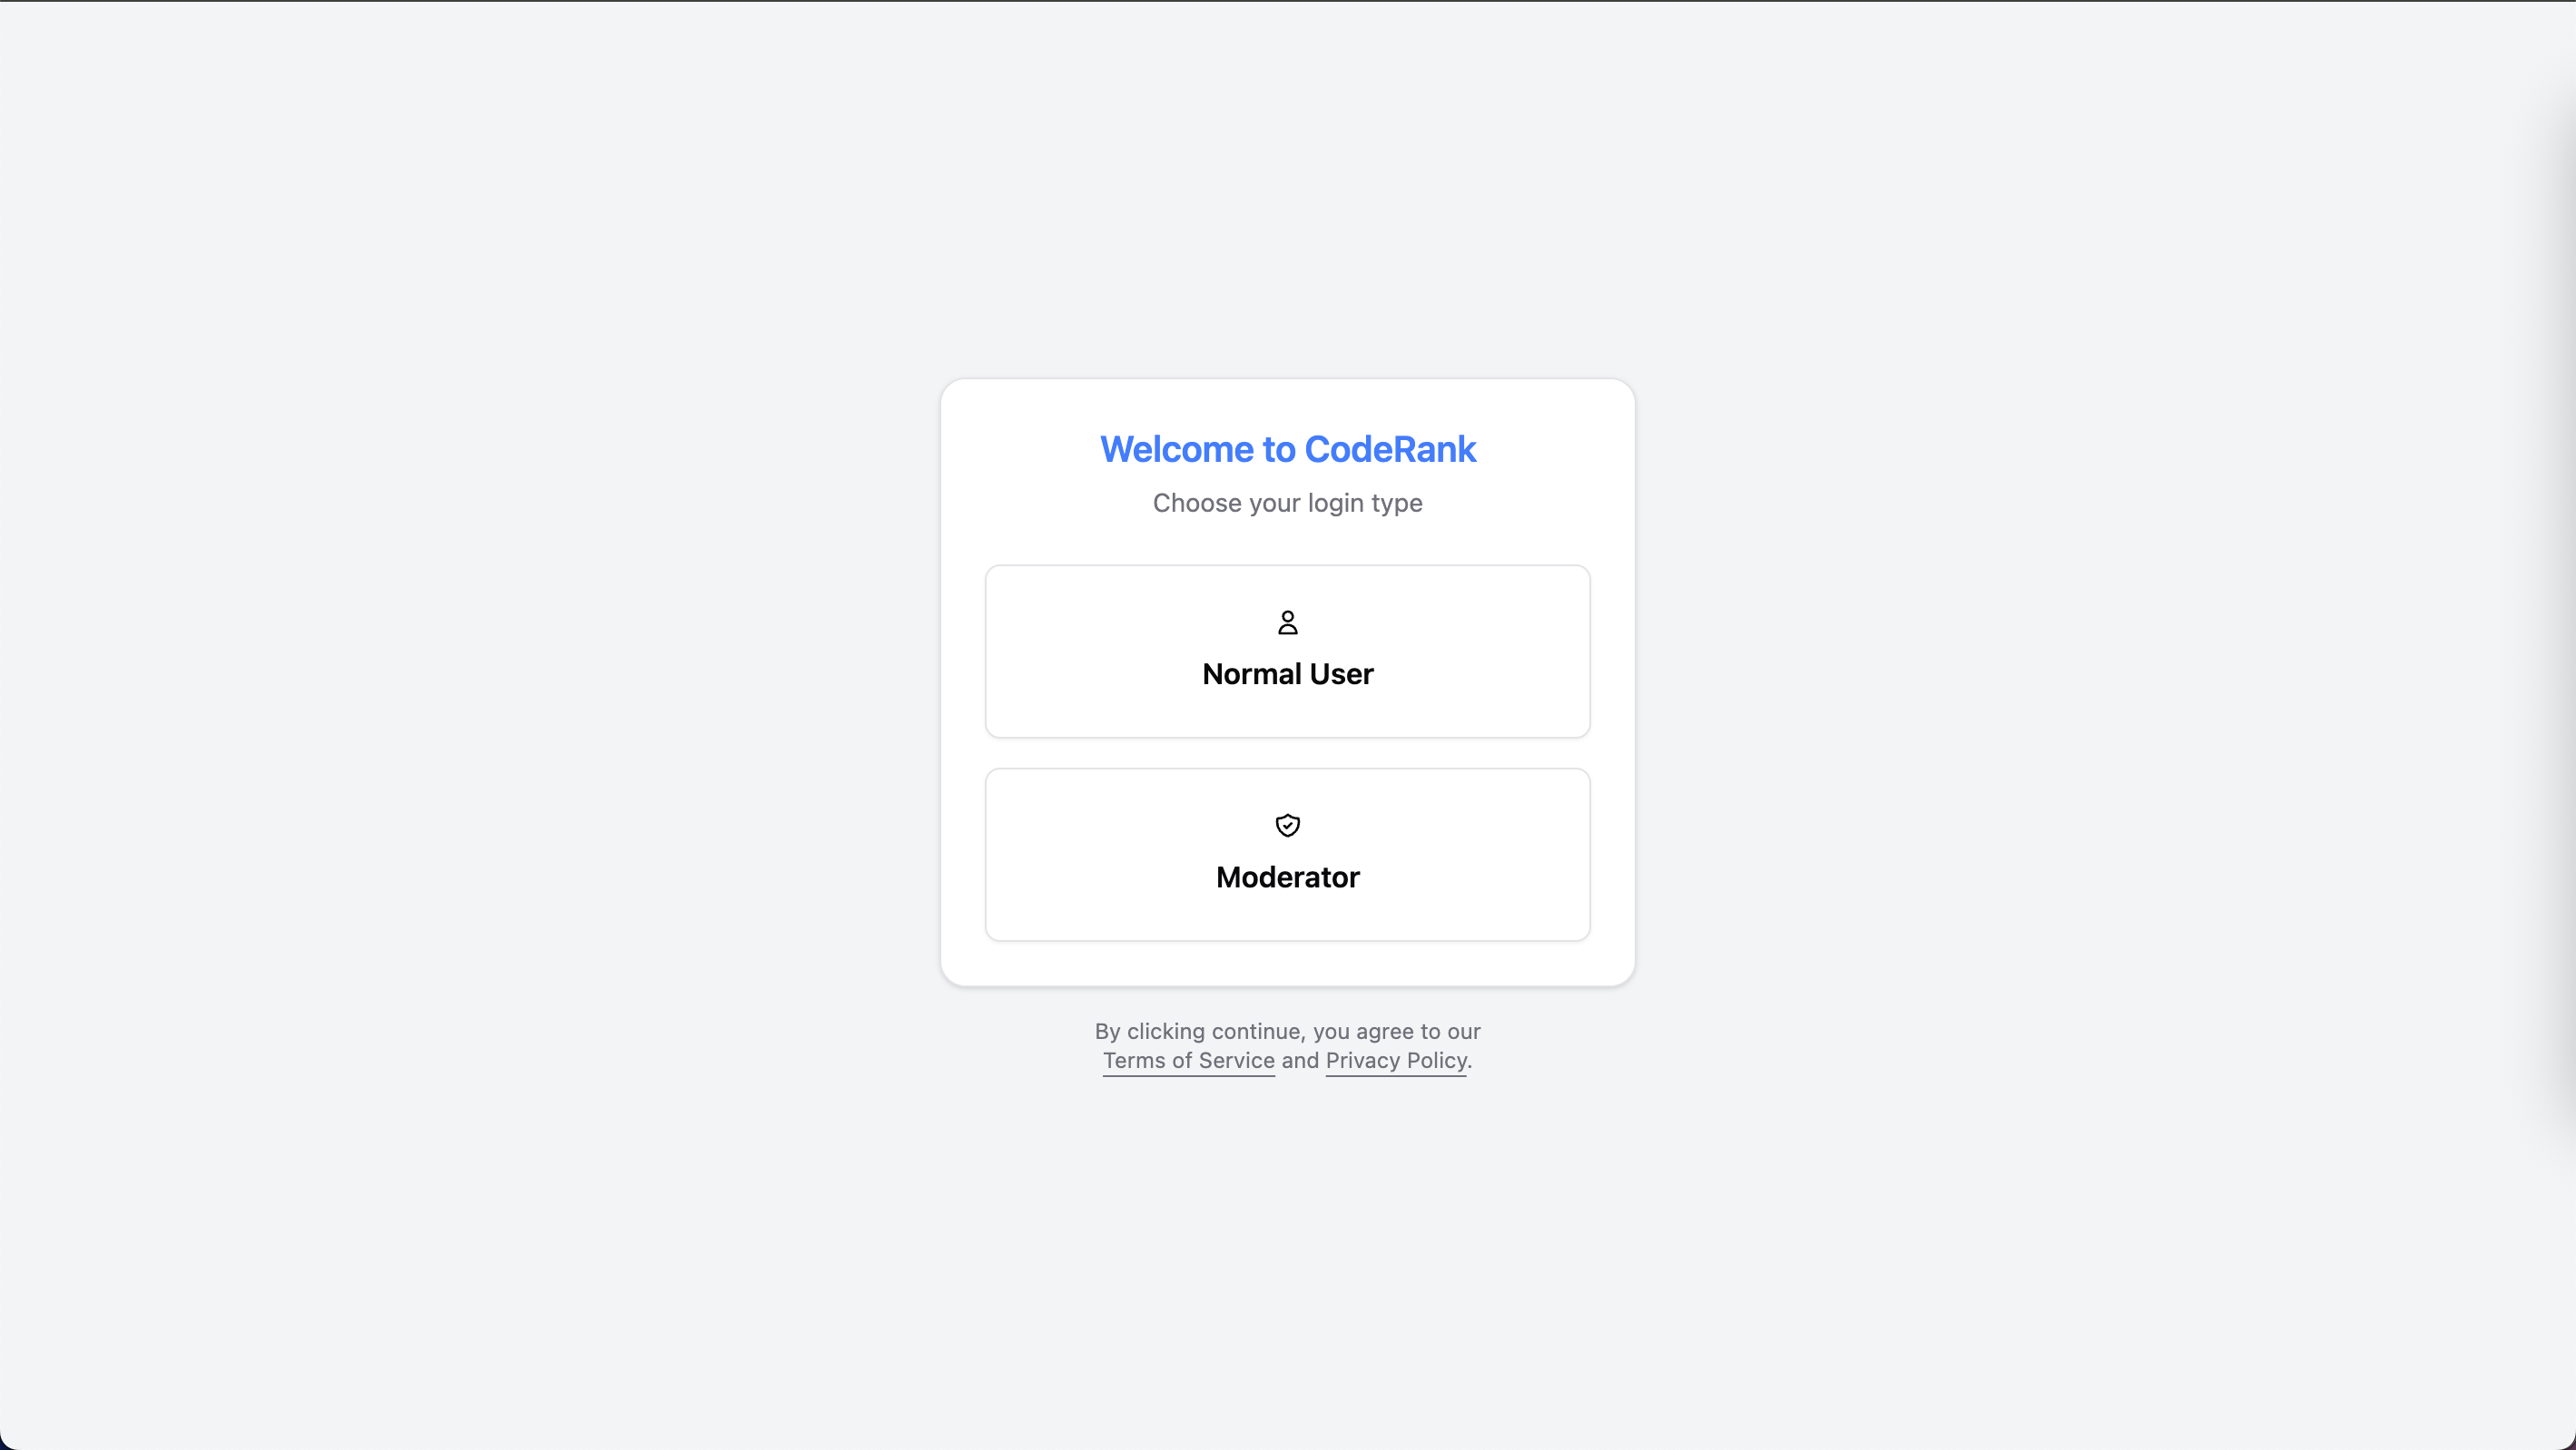
\includegraphics[width=1\textwidth]{Contents/Chapter 3/Wireframe/Primary User/login_selection.png}
    \vspace{0.6cm}
    \caption{Login Page \- Role Selection}
\end{figure}

For Primary User, after selecting User login, the user will be directed to the User Login Page. This will include fields for entering username and password, along with a login button. There is also an option for login vie Google OAuth. After login successful, there will be a toast notification indicating success and redirecting to the Problem List page. Any validation errors will be displayed in the below of the corresponding input fields if the user enters incorrect credentials.
\begin{figure}[H]
    \centering
    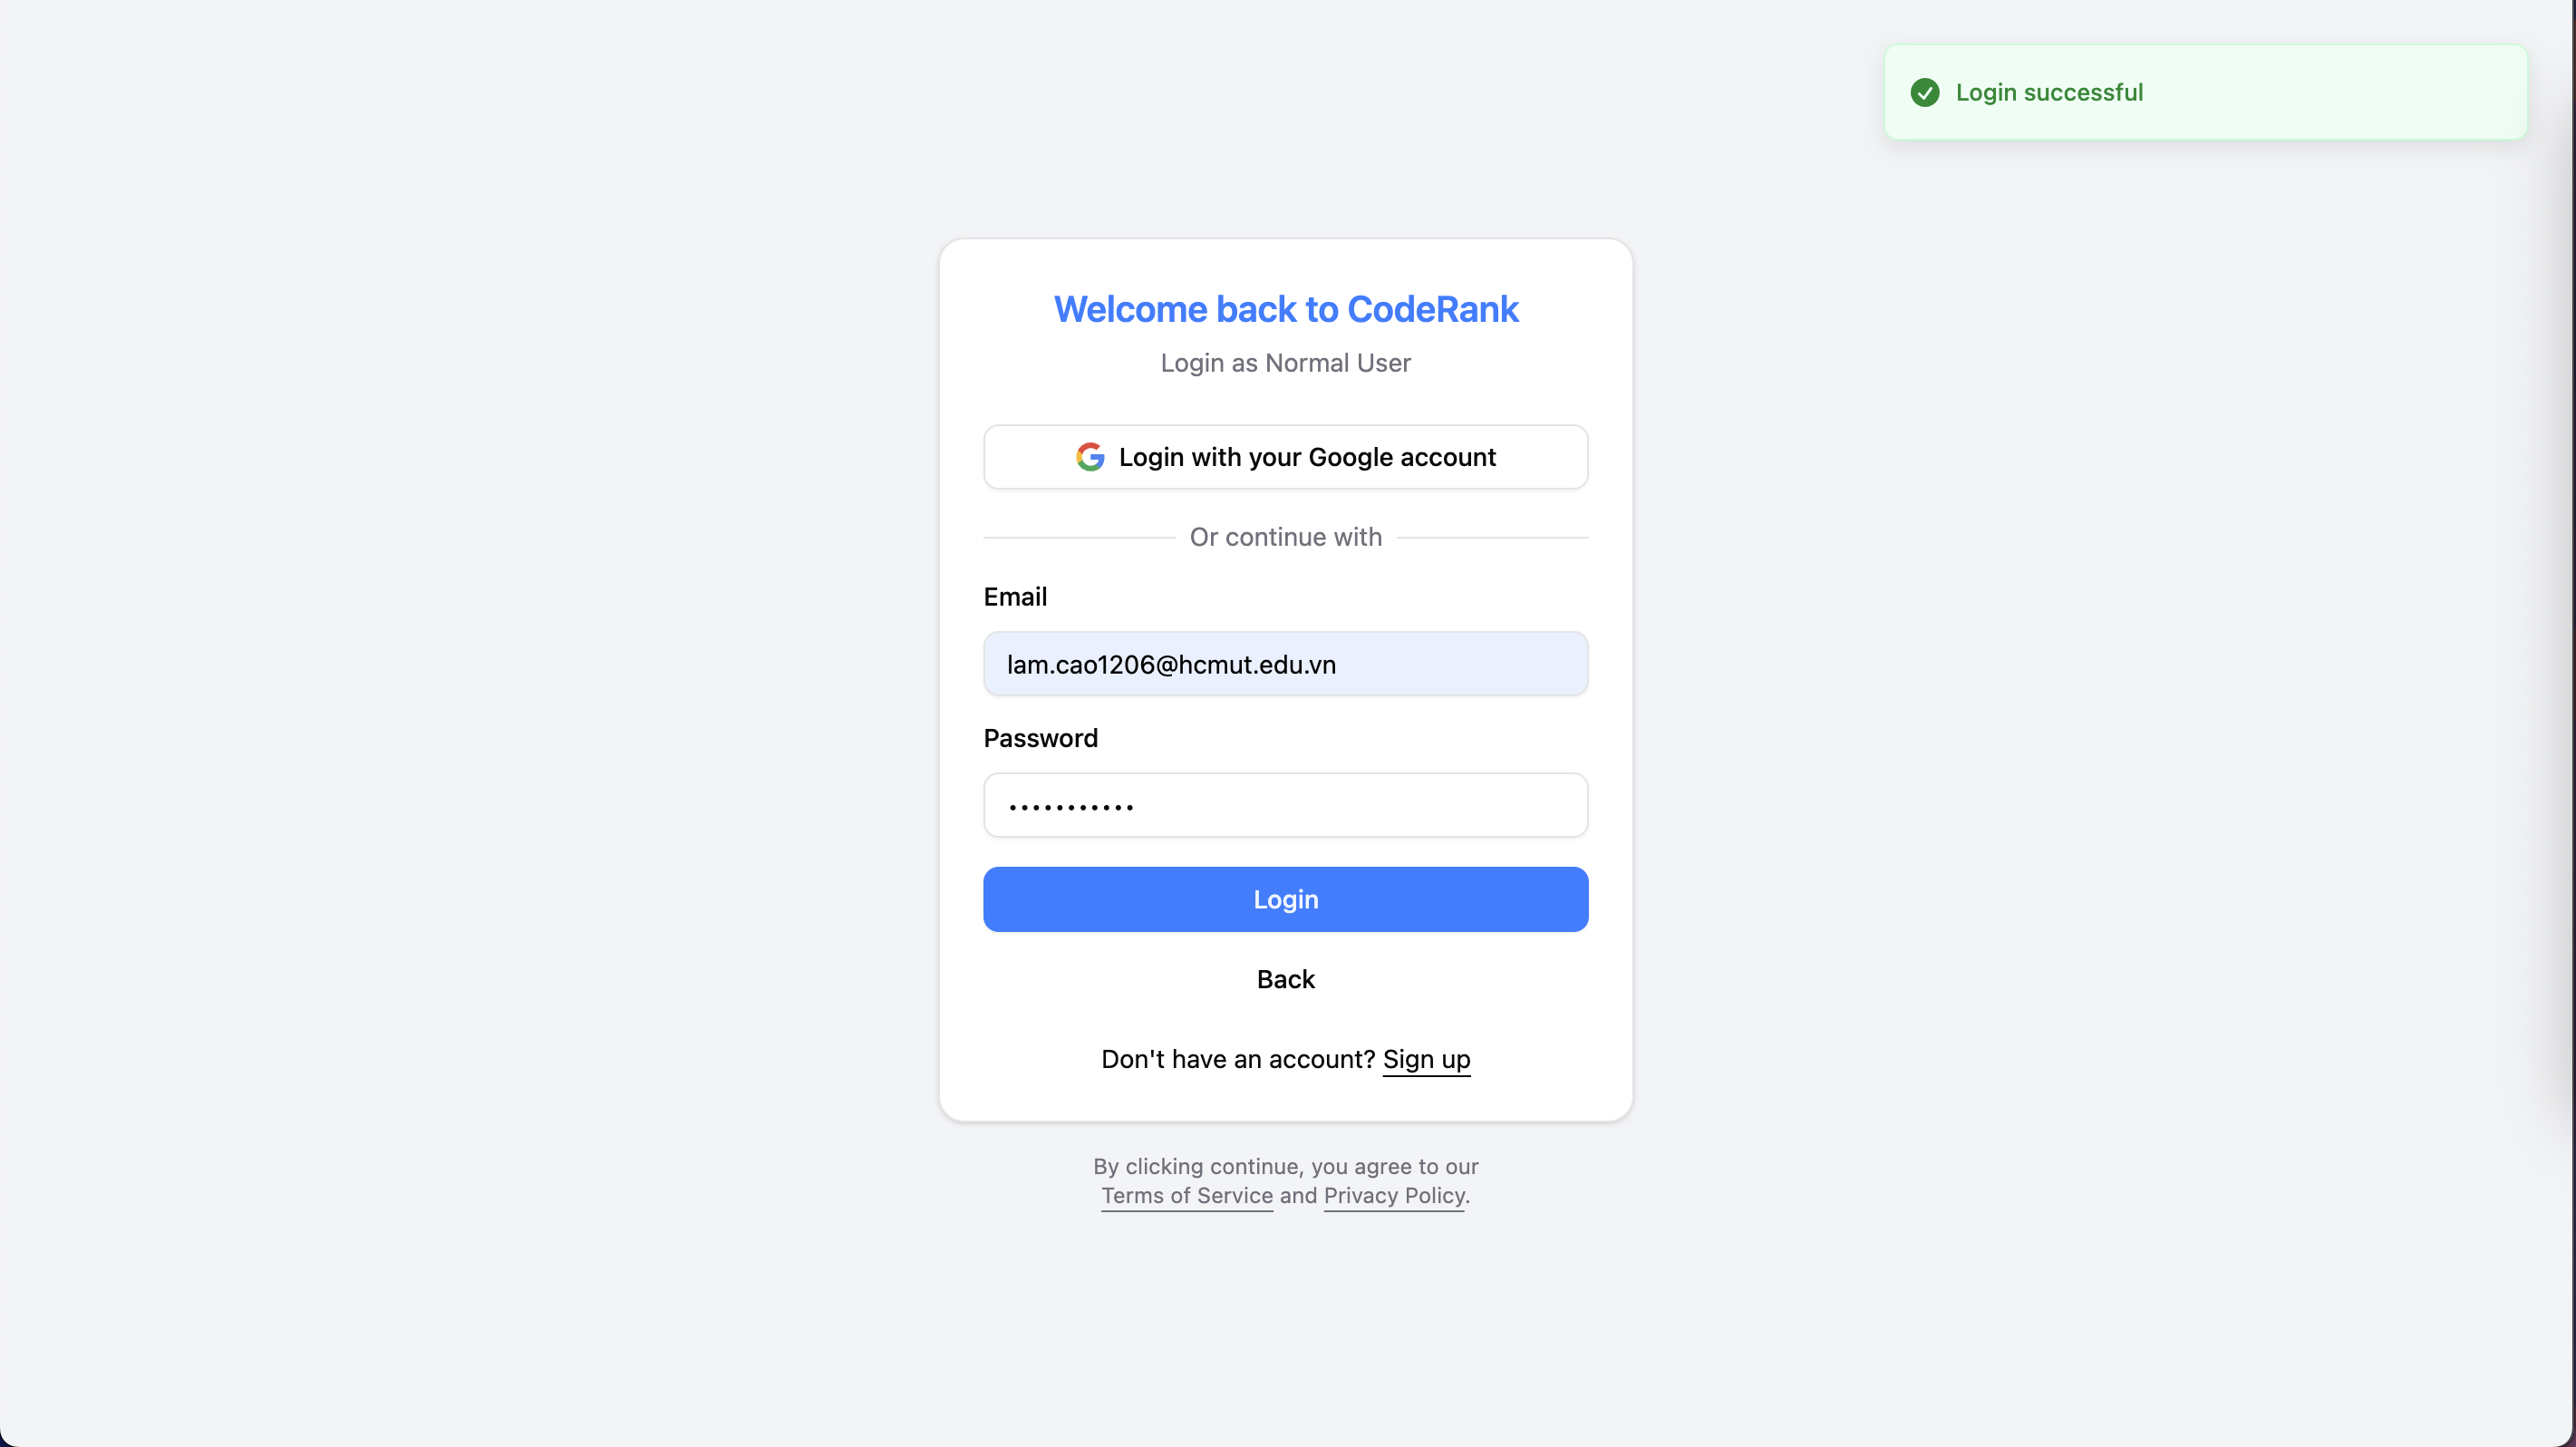
\includegraphics[width=1\textwidth]{Contents/Chapter 3/Wireframe/Primary User/login_primary.png}
    \vspace{0.6cm}
    \caption{Login Page \- Primary User Login}
\end{figure}

\subsubsubsection*{Problem List}
After logging in, the Primary User will be directed to the Problem List page. This page displays a list of coding problems available on the platform, along with relevant details such as problem title, difficulty level, and tags. Users can filter and sort the problems based on various criteria to find specific challenges they want to solve.
\begin{figure}[H]
    \centering
    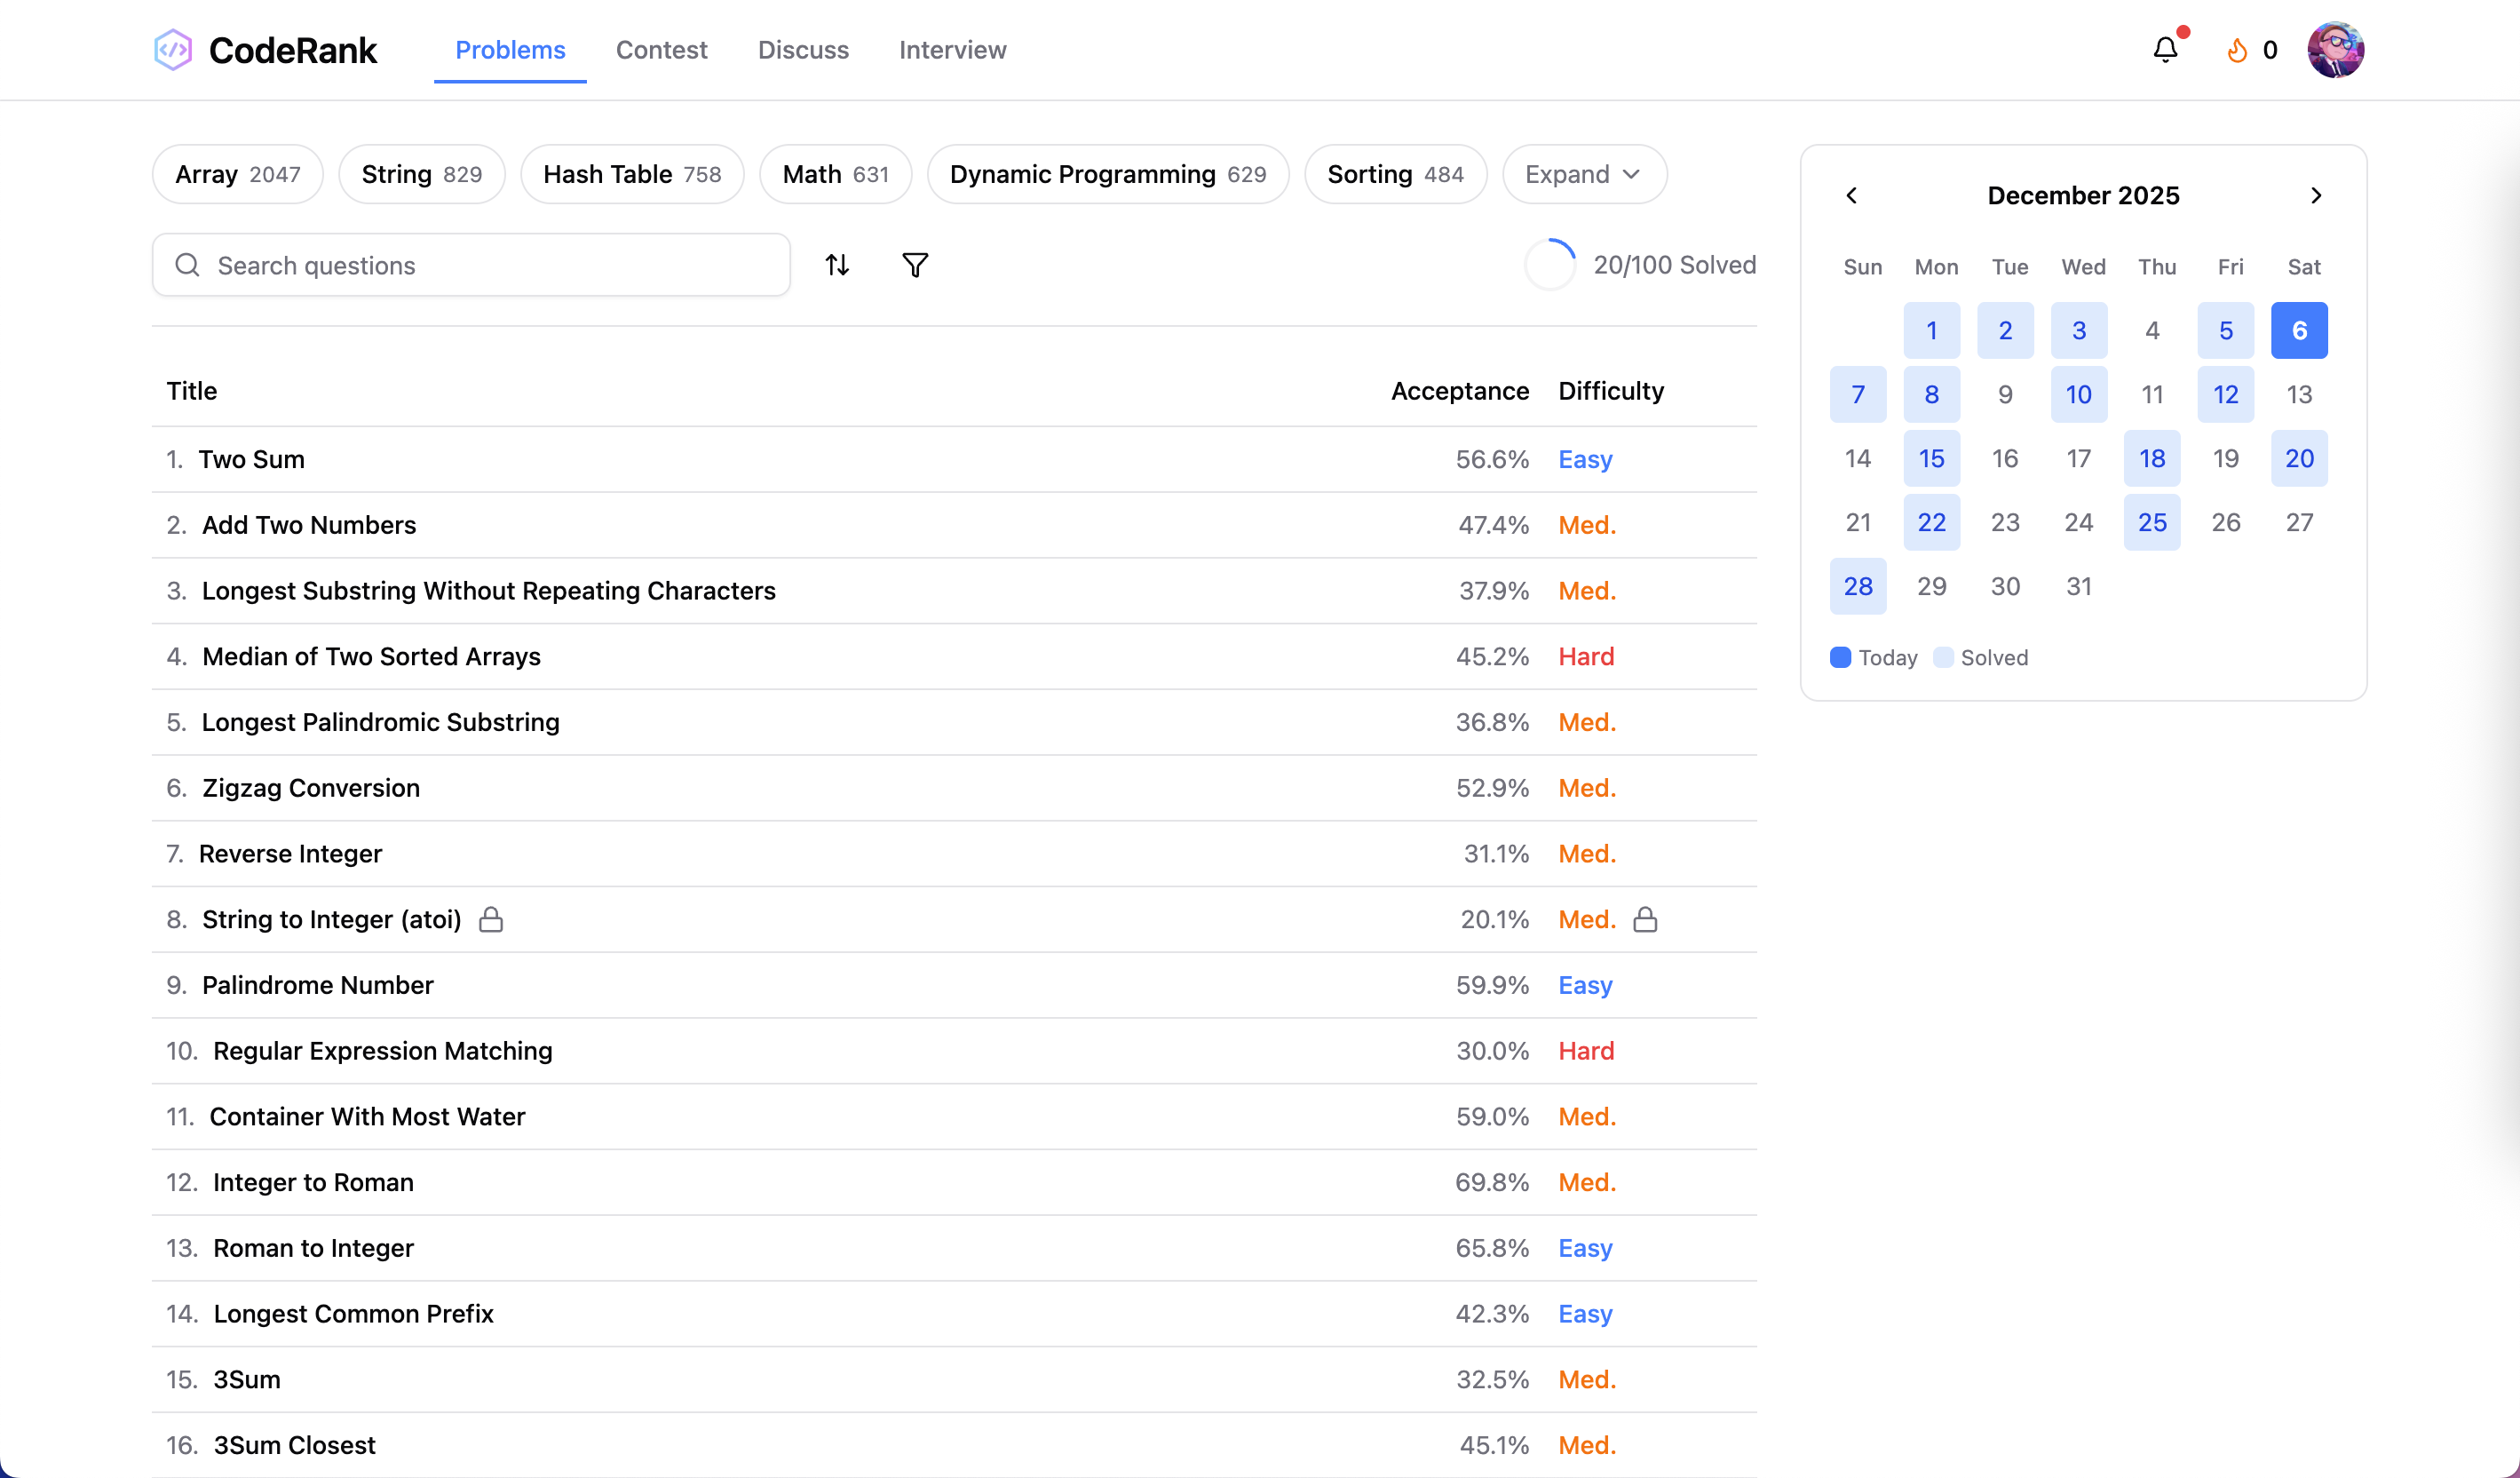
\includegraphics[width=1\textwidth]{Contents/Chapter 3/Wireframe/Primary User/problem_list.png}
    \vspace{0.6cm}
    \caption{Problem List page}
\end{figure}

The Problem List page also includes a search bar at the top, allowing users to quickly search for problems by keywords or tags. Each problem entry in the list is clickable, leading to the Problem Detail page where users can view the full problem description and submit their solutions.
\begin{figure}[H]
    \centering
    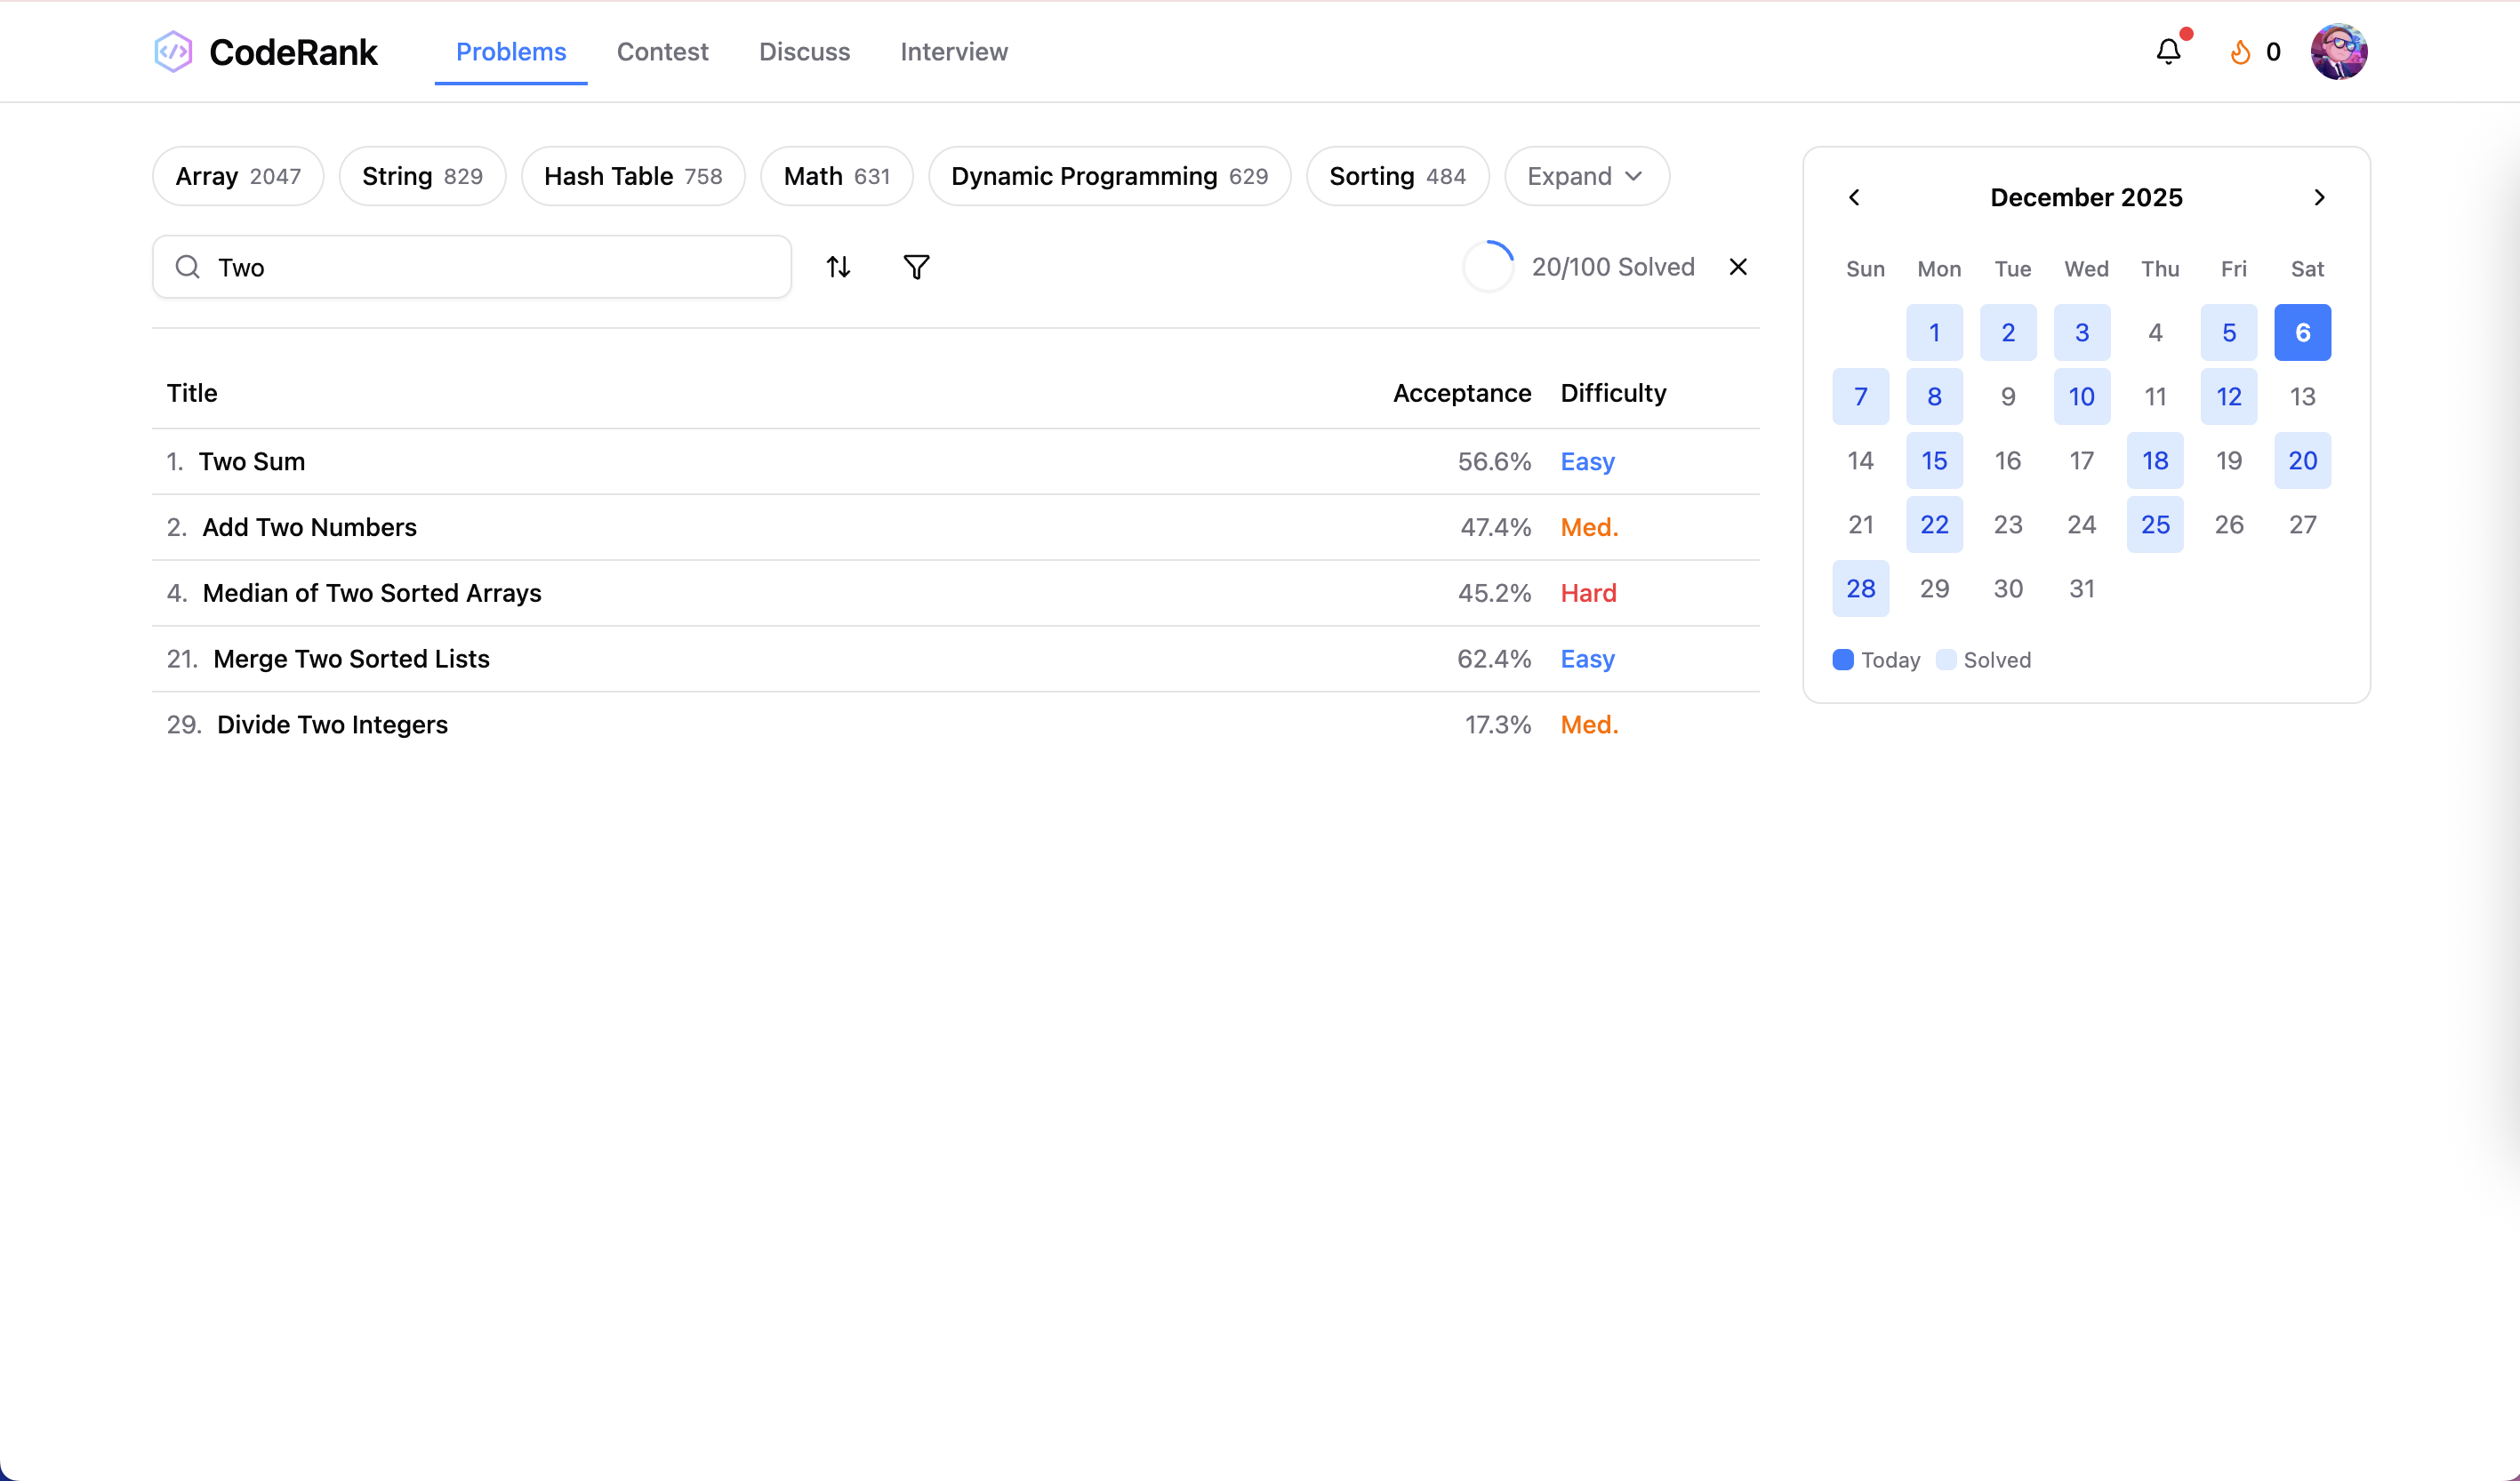
\includegraphics[width=1\textwidth]{Contents/Chapter 3/Wireframe/Primary User/problem_list_search.png}
    \vspace{0.6cm}
    \caption{Problem List Search}
\end{figure}

In order to solve a problem, the user can click on the problem title in the Problem List. This will take them to the Problem Detail page, where they can read the problem description, view constraints, and submit their code solution.
\begin{figure}[H]
    \centering
    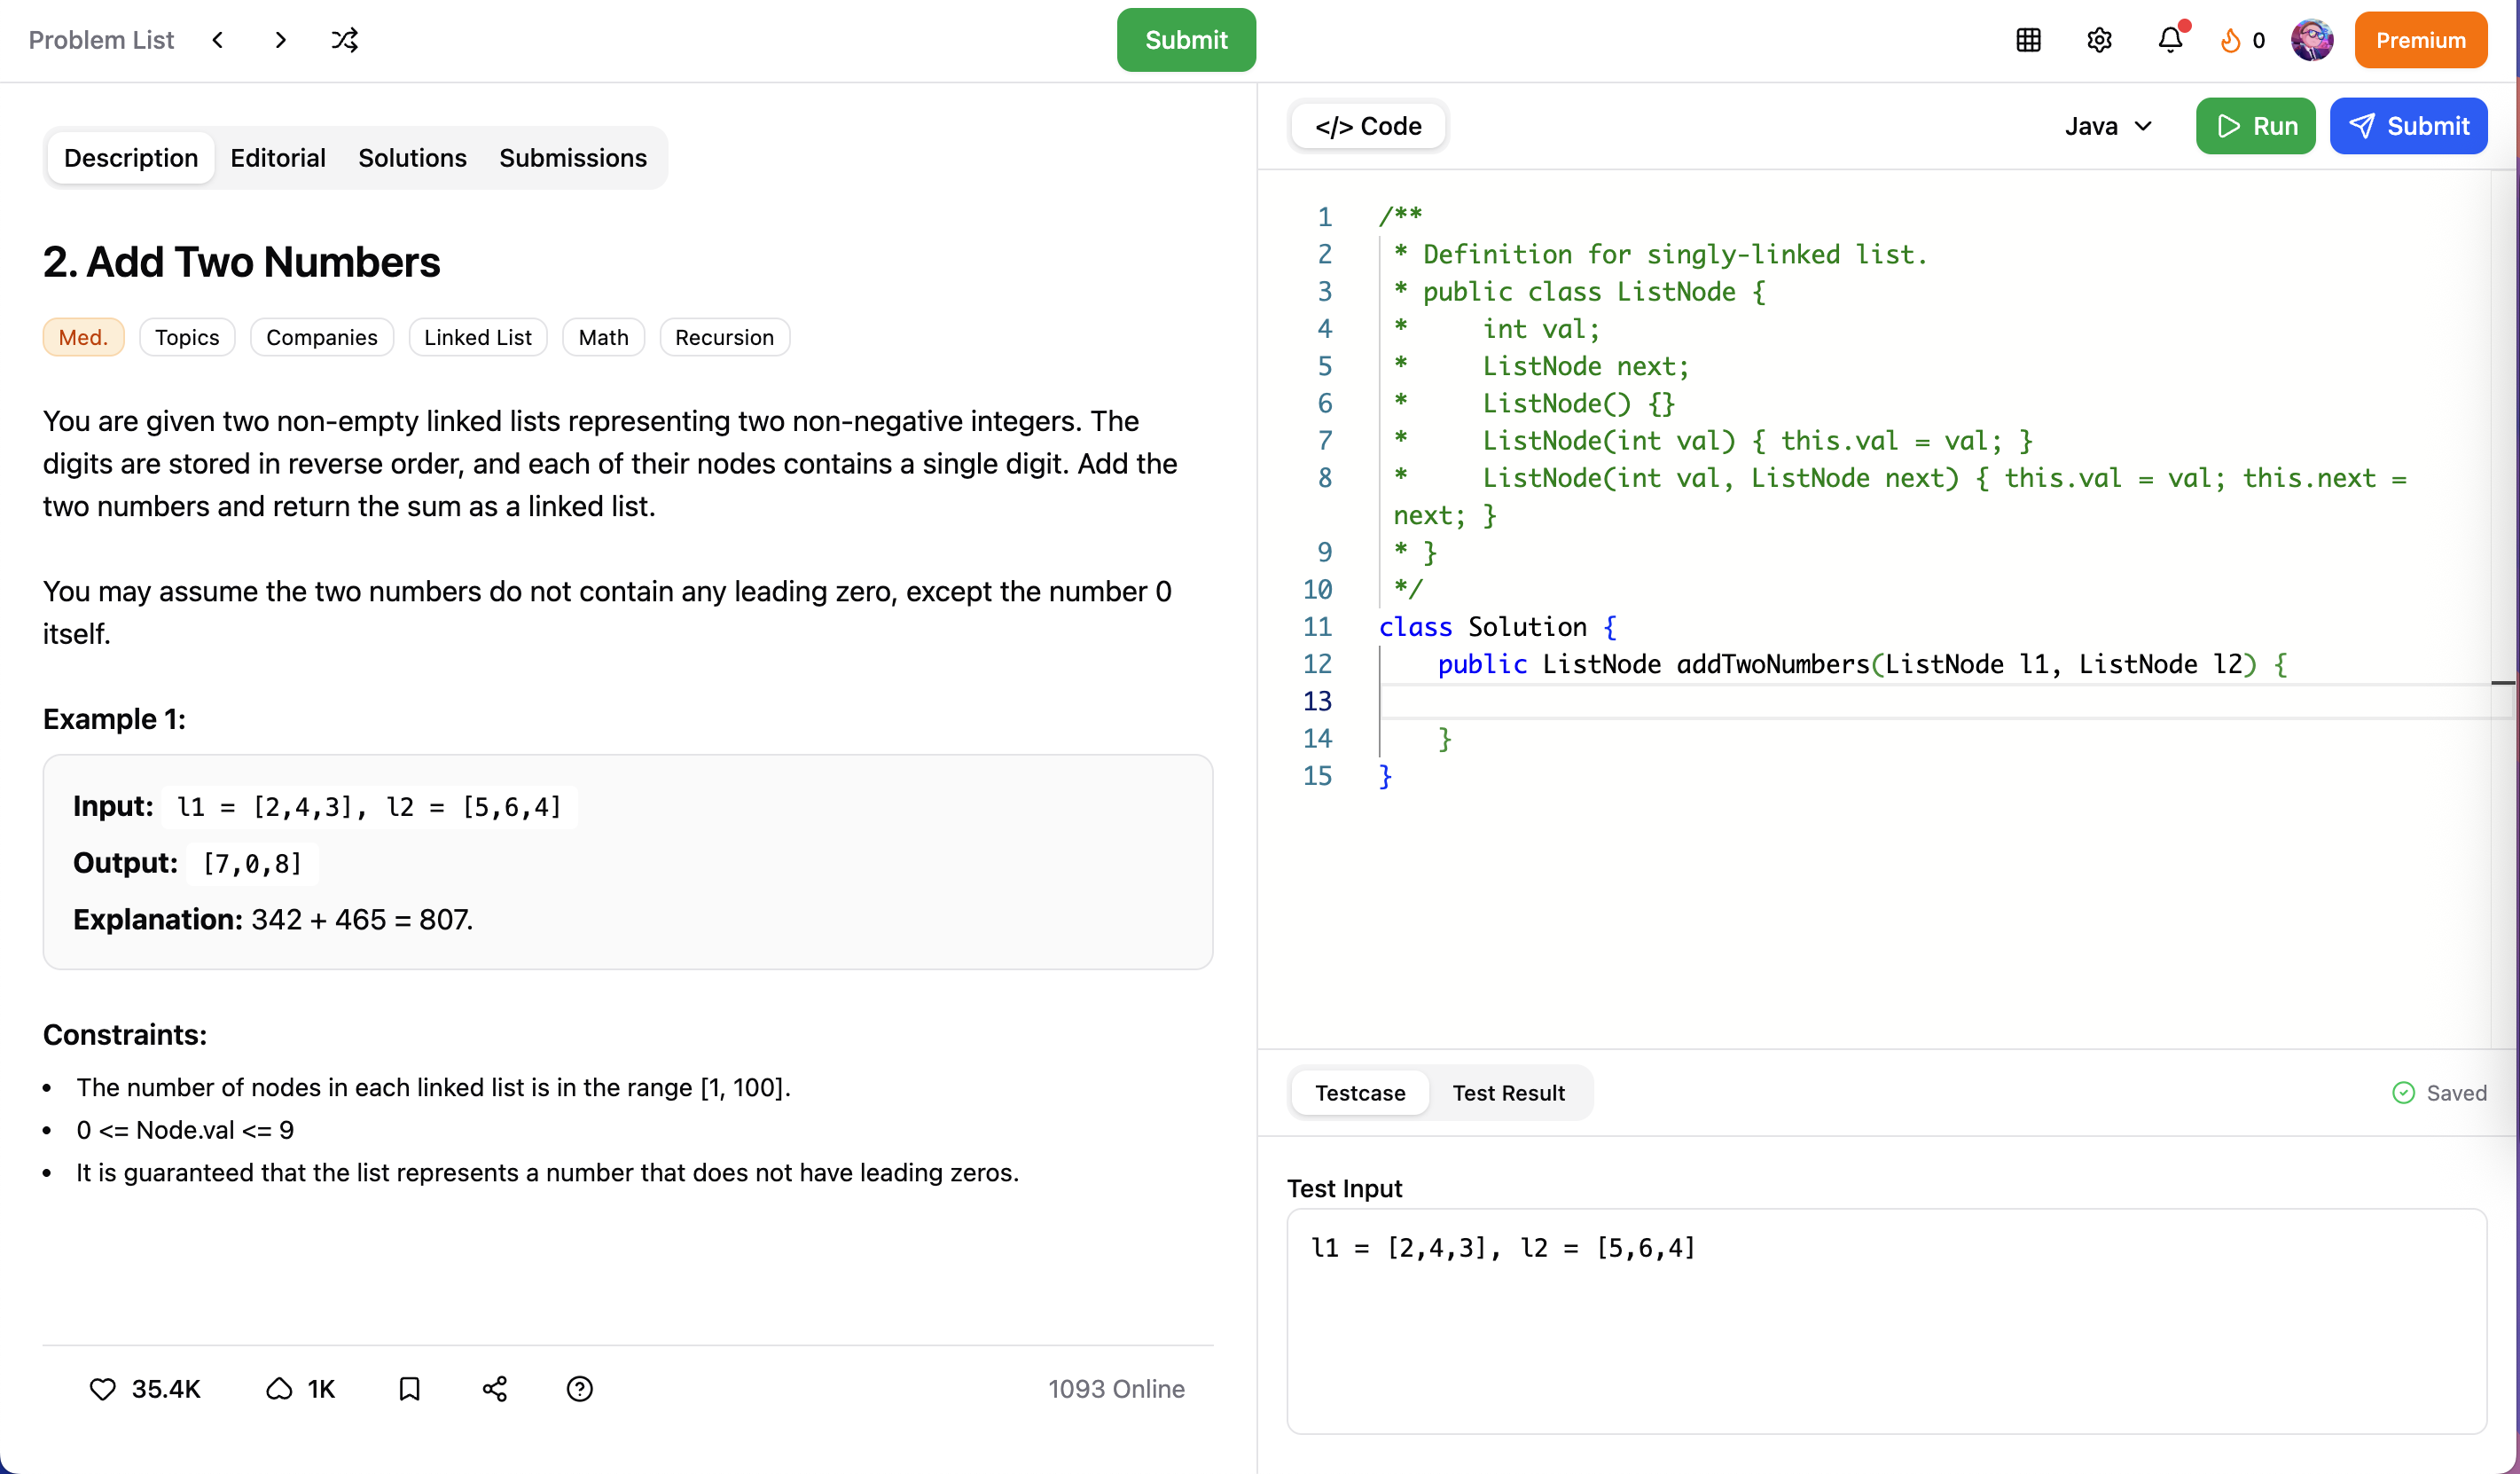
\includegraphics[width=1\textwidth]{Contents/Chapter 3/Wireframe/Primary User/problem_detail.png}
    \vspace{0.6cm}
    \caption{Problem Detail page}
\end{figure}


\subsubsection*{Discussion}

Beside solving problems, primary user can access the Discussion feature from the main navigation menu after logging in. The Discussion feature allows users to engage in conversations related to coding problems, share insights, ask questions, and collaborate with other users.

\begin{figure}[H]
    \centering
    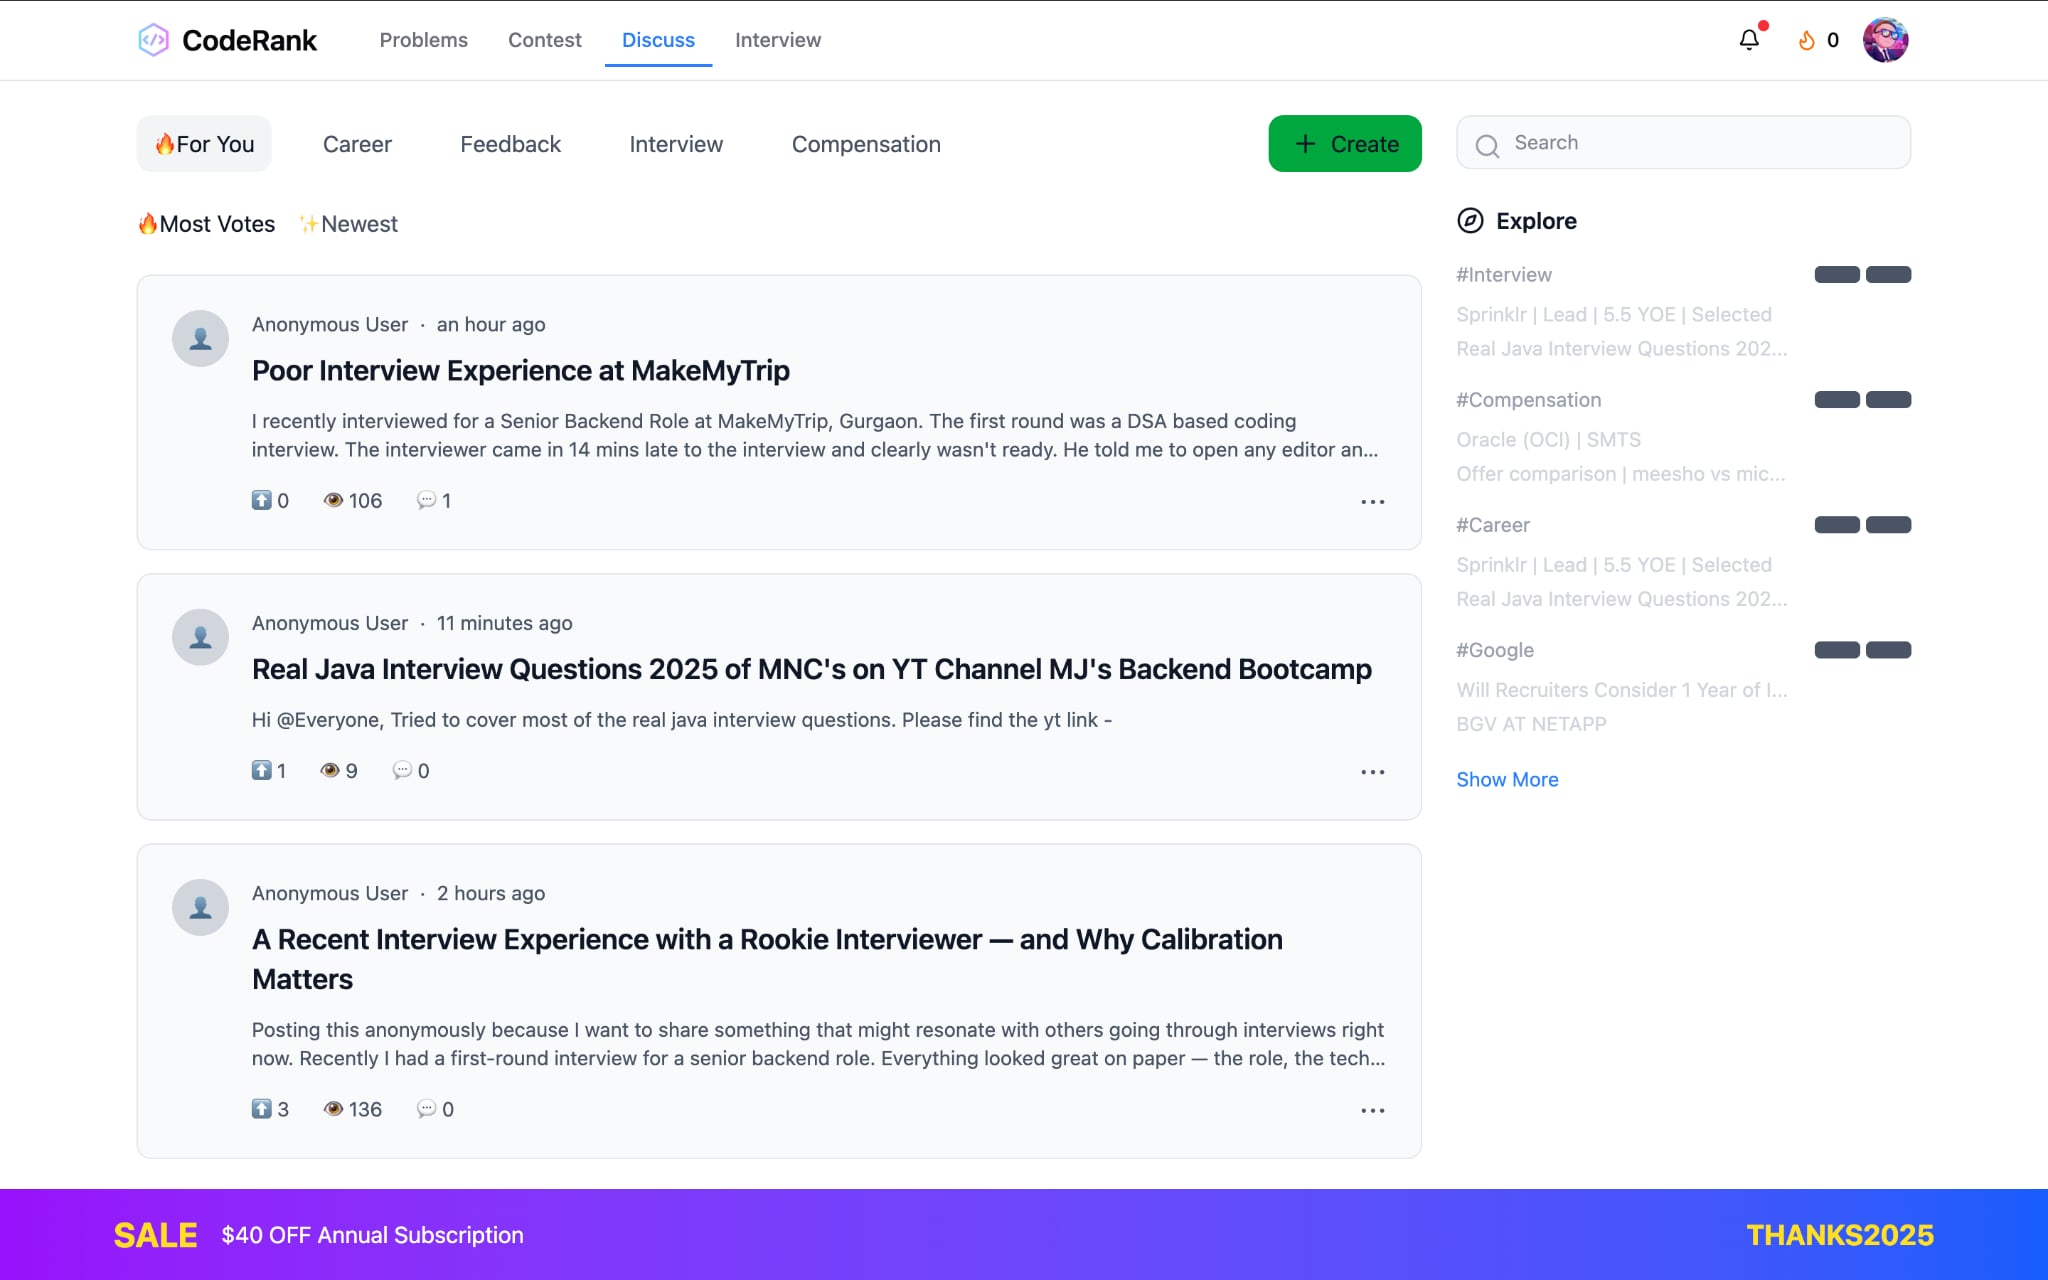
\includegraphics[width=1\textwidth]{Contents/Chapter 3/Wireframe/Primary User/discussion-1.jpeg}
    \vspace{0.6cm}
    \caption{Discussion List}
\end{figure}

In order to join a discussion, the user can select a specific discussion thread from the Discussion List. This will take them to the Discussion Detail page, where they can view all messages within that thread and participate in the conversation by posting their own messages.
\begin{figure}[H]
    \centering
    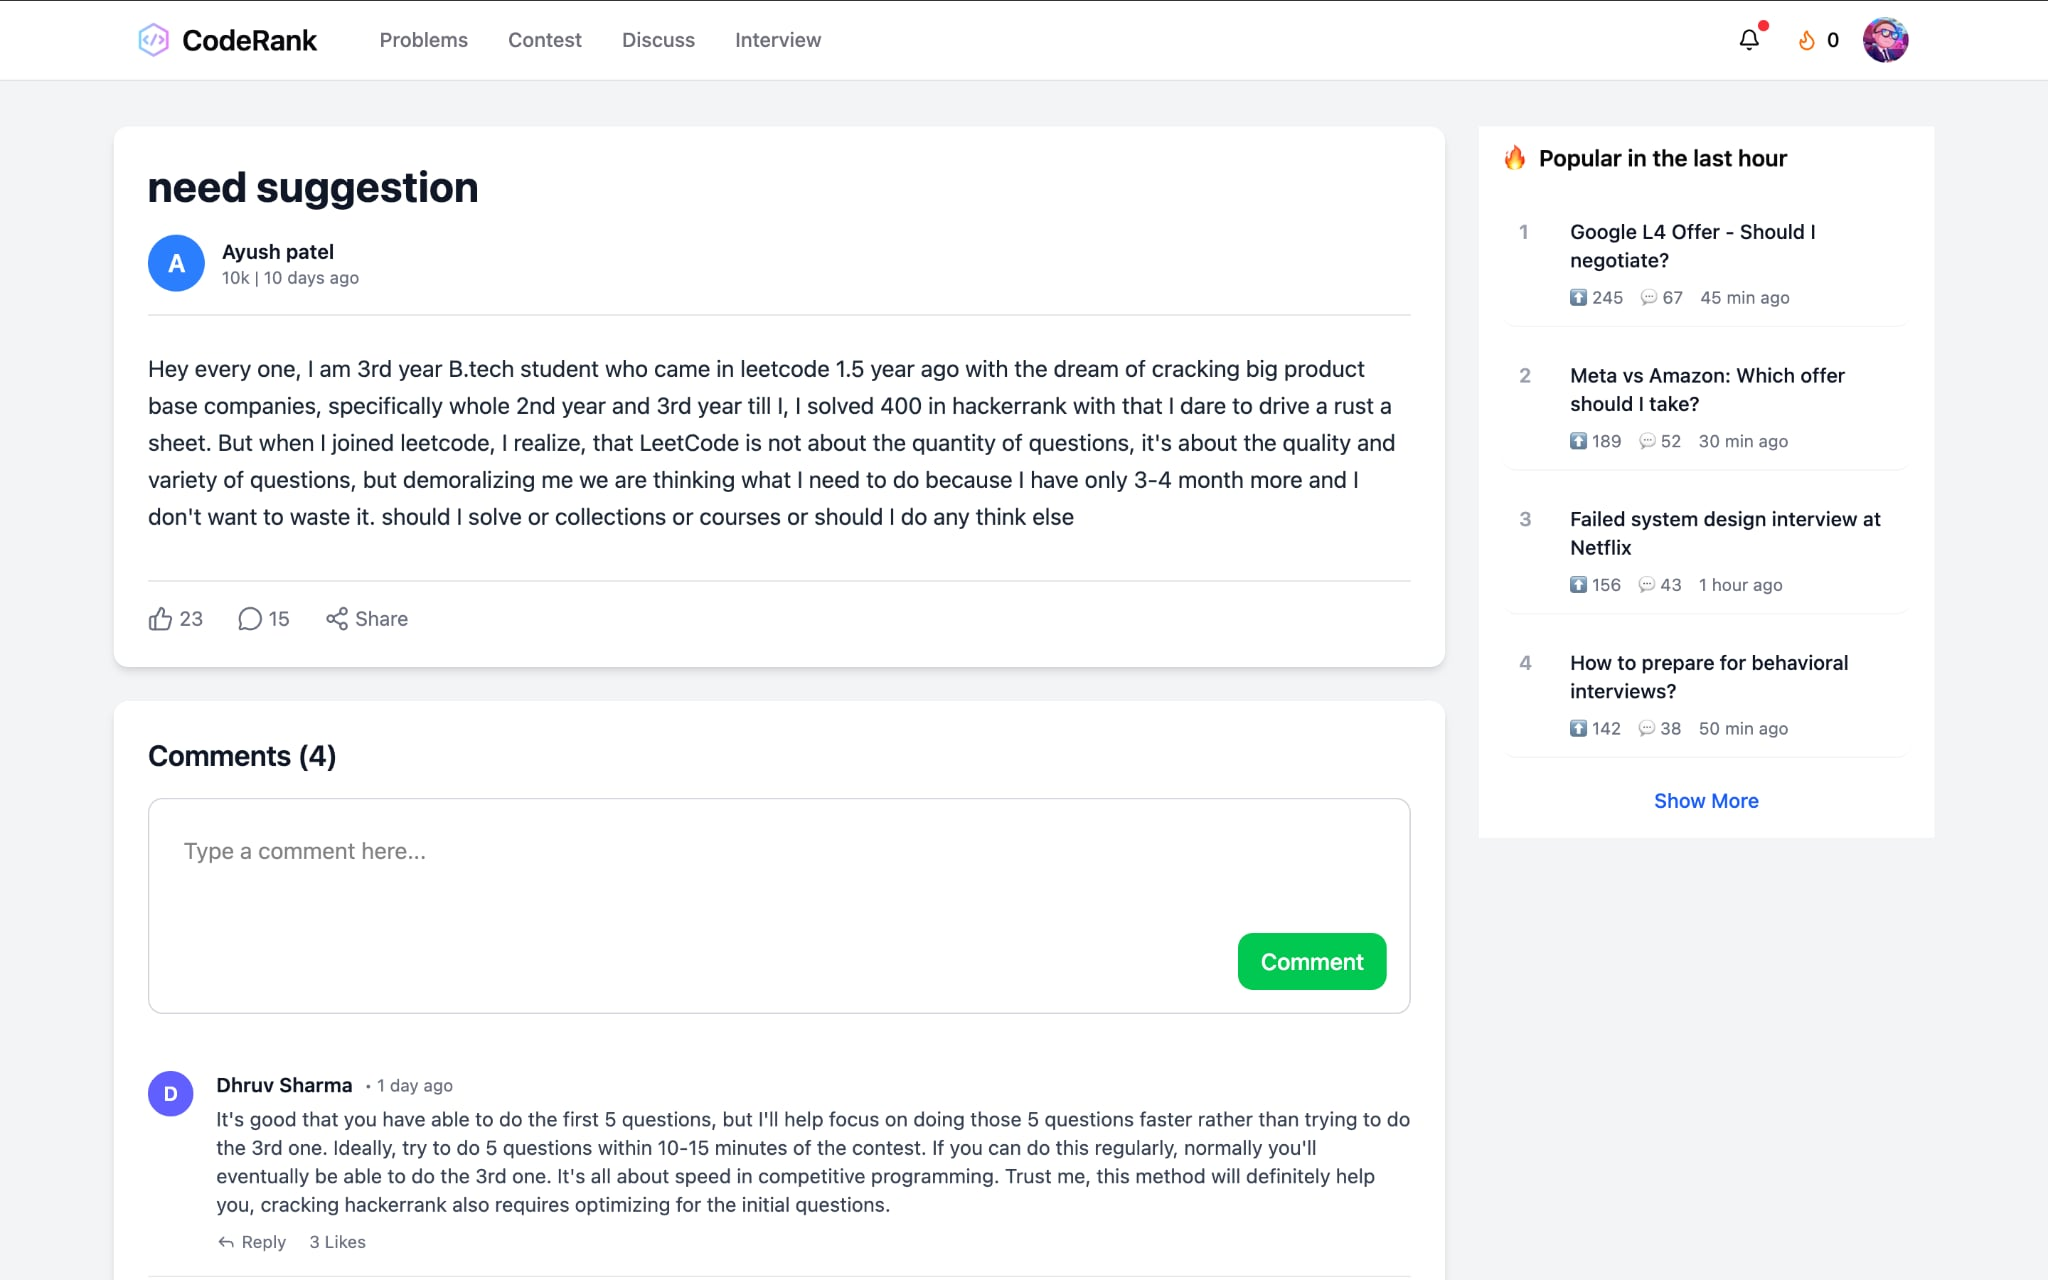
\includegraphics[width=1\textwidth]{Contents/Chapter 3/Wireframe/Primary User/discussion-3.jpeg}
    \vspace{0.6cm}
    \caption{Discussion Detail}
\end{figure}

To create a new discussion thread, the user can click in the button \textbf{Create} in the discussion list page. Here, they can enter a title, choose topic, tags, and write the initial message to start the discussion.

\begin{figure}[H]
    \centering
    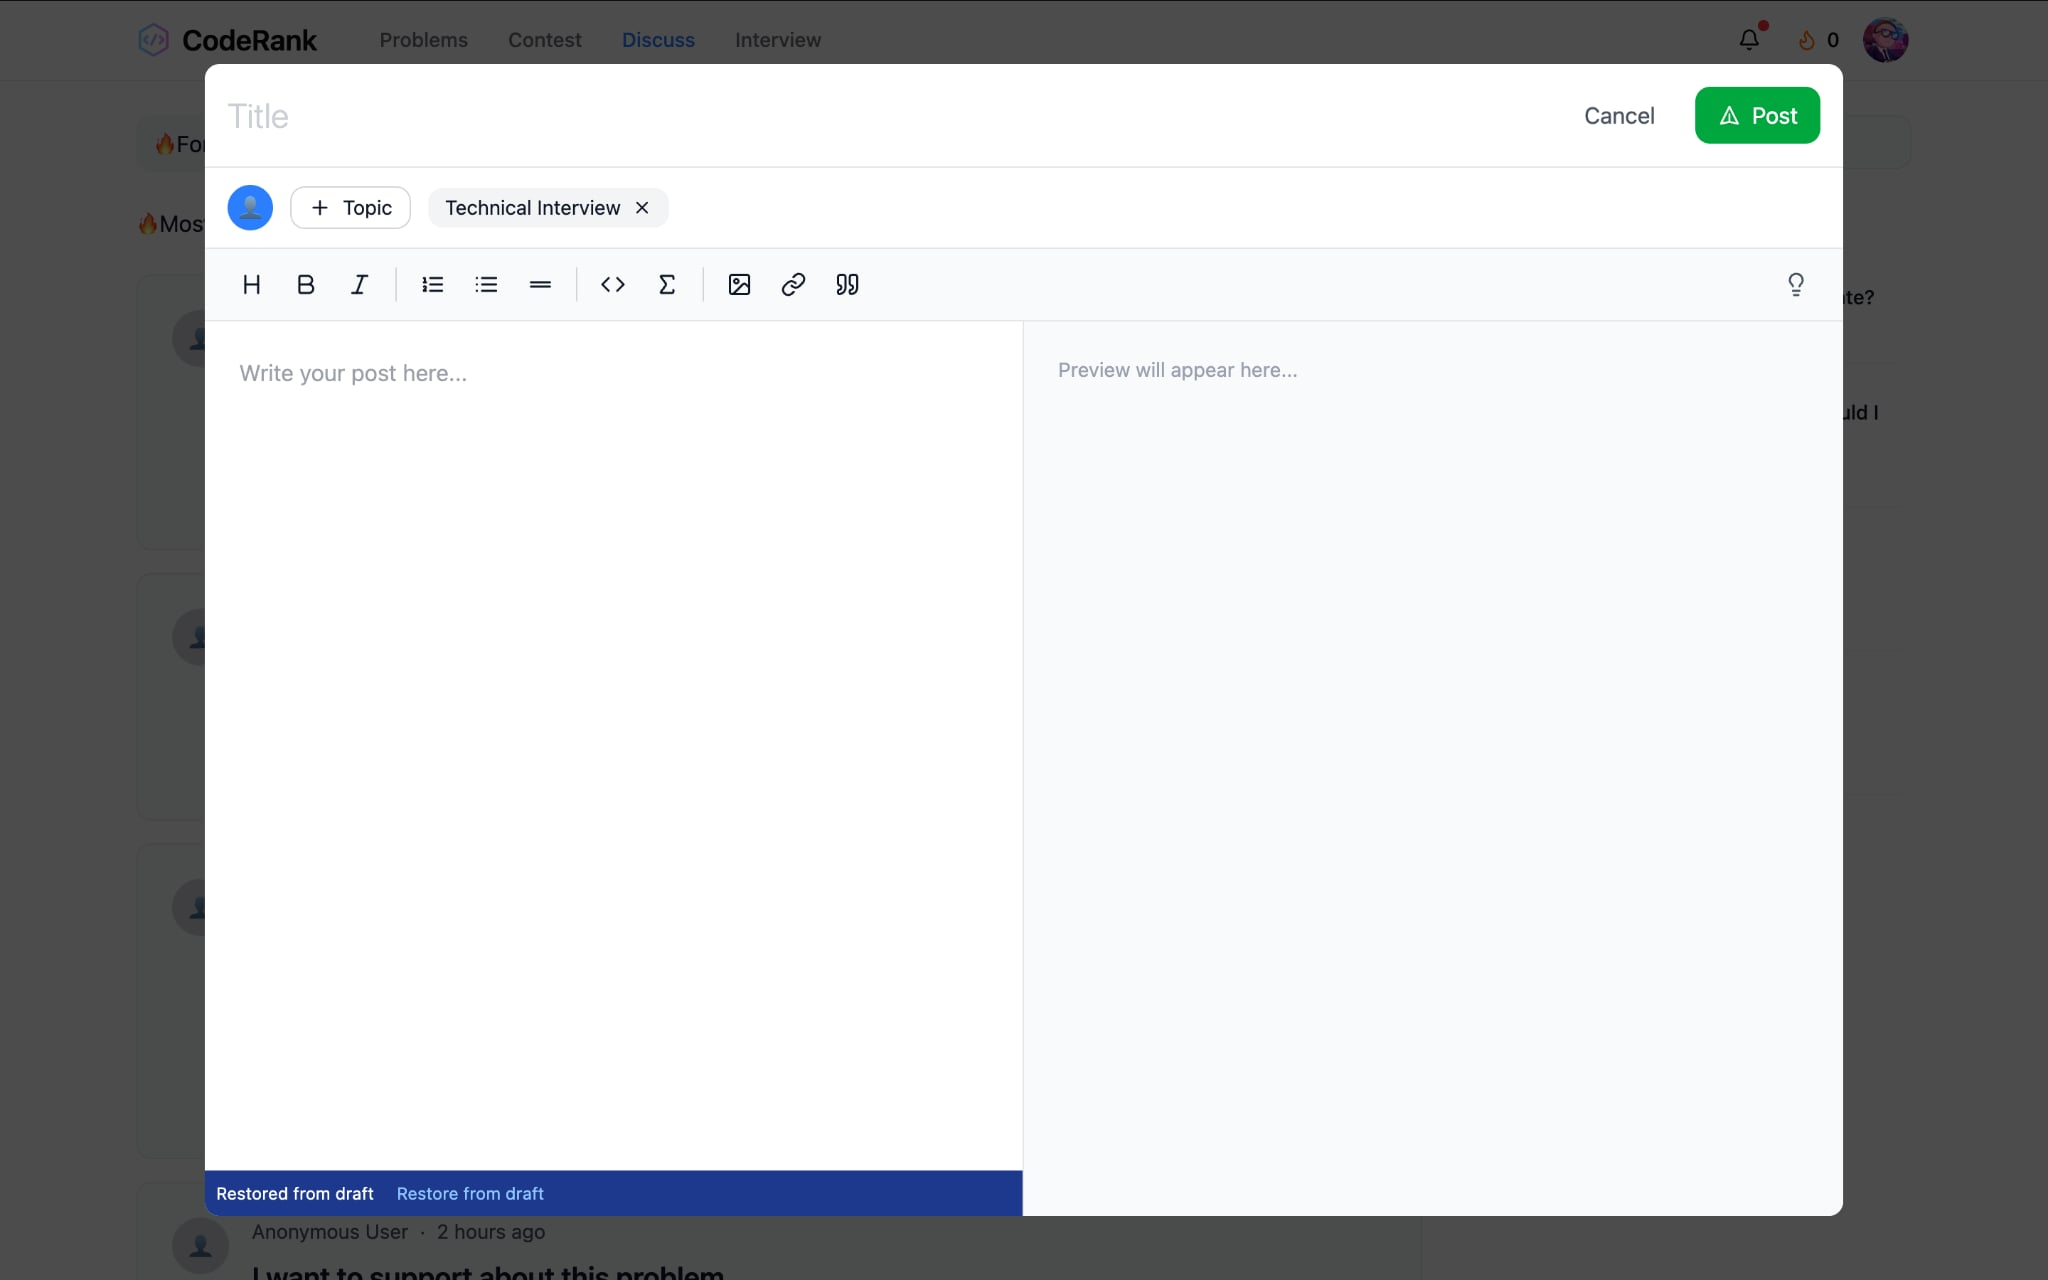
\includegraphics[width=1\textwidth]{Contents/Chapter 3/Wireframe/Primary User/discussion-2.jpeg}
    \vspace{0.6cm}
    \caption{Create Discussion}
\end{figure}

\subsubsection*{Contest Participation}

Primary users can participate in coding contests hosted on the platform by navigating to the Contest List page from the main navigation menu. This page displays a list of upcoming and ongoing contests, along with relevant details such as contest name, start time, end time, and duration.
\begin{figure}[H]
    \centering
    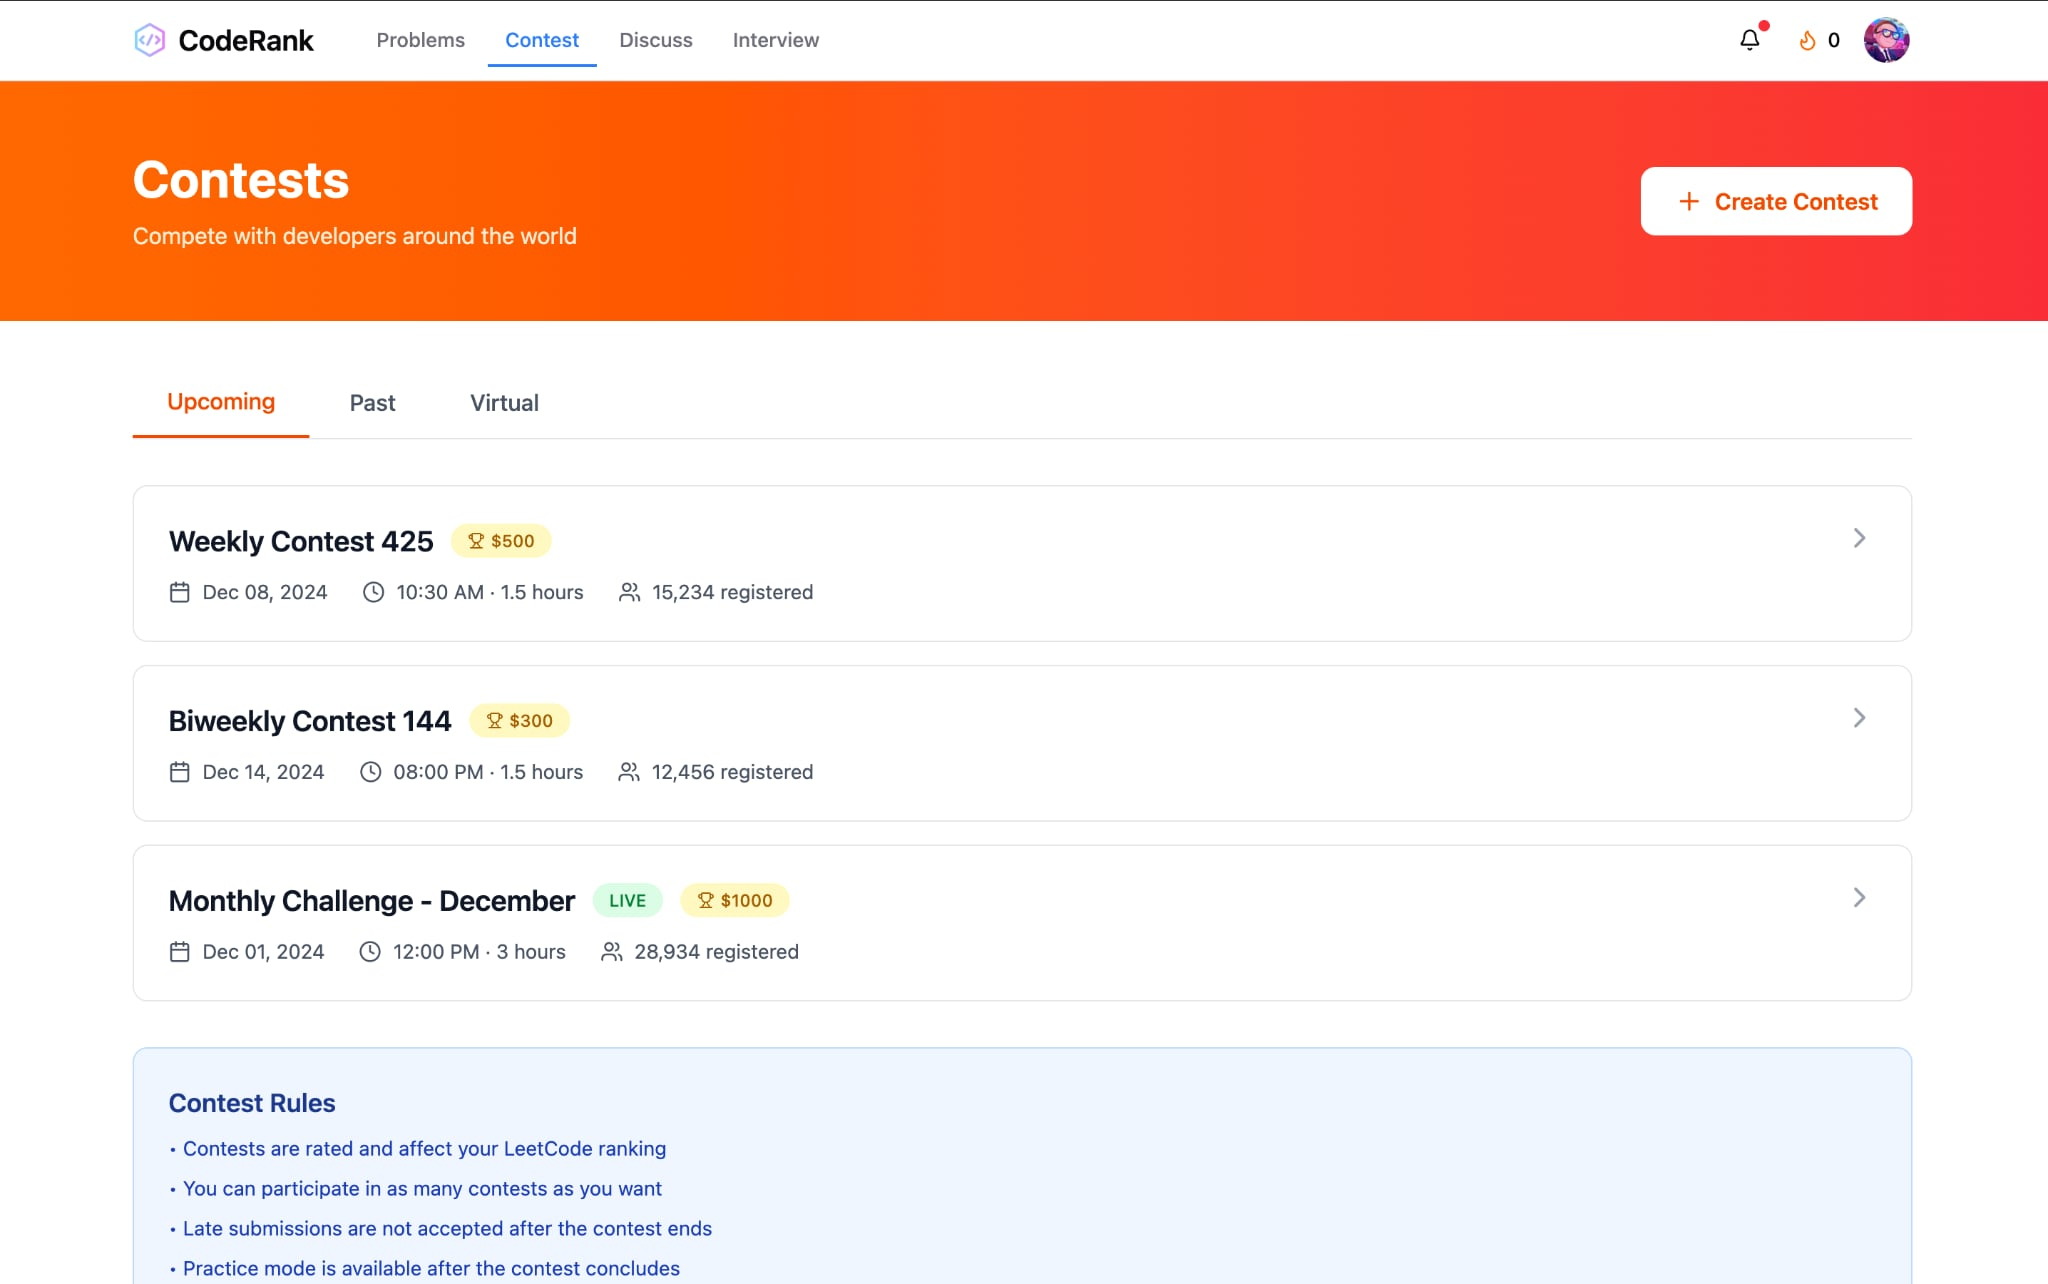
\includegraphics[width=1\textwidth]{Contents/Chapter 3/Wireframe/Primary User/contest-1.jpeg}
    \vspace{0.6cm}
    \caption{Contest List}
\end{figure}

In order to view the details of a specific contest, the user can click on the contest name in the Contest List. This will take them to the Contest Detail page, where they can see the information about the contest, including the list of problems included in the contest and the rules for participation.
\begin{figure}[H]
    \centering
    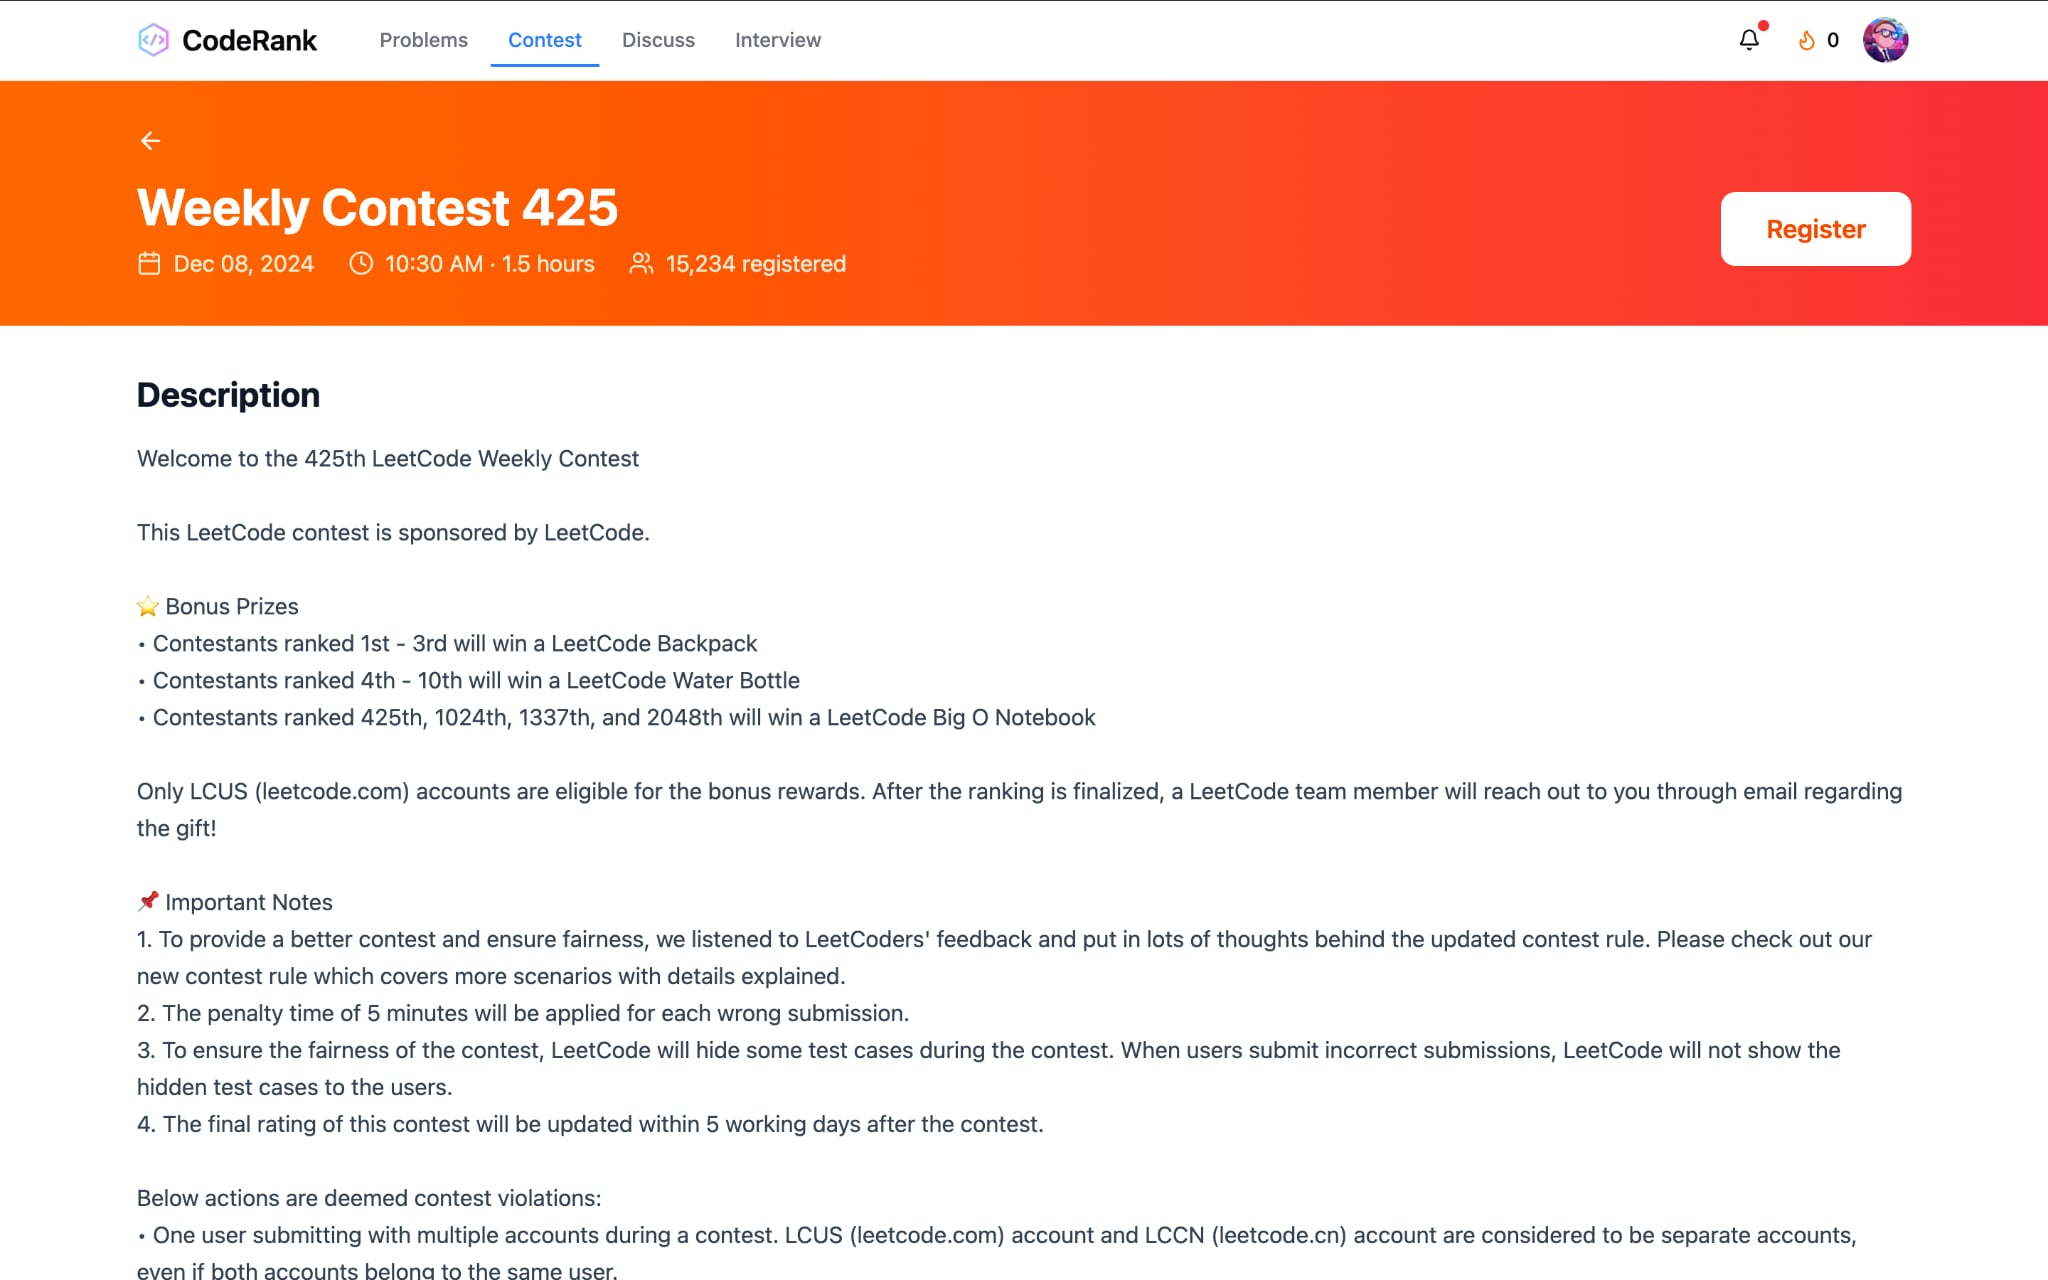
\includegraphics[width=1\textwidth]{Contents/Chapter 3/Wireframe/Primary User/contest-3.jpeg}
    \vspace{0.6cm}
    \caption{Contest Detail}
\end{figure}

After the contest ended, user can view the leaderboard to see their ranking and performance compared to other participants by scrolling down below the contest detail.
\begin{figure}[H]
    \centering
    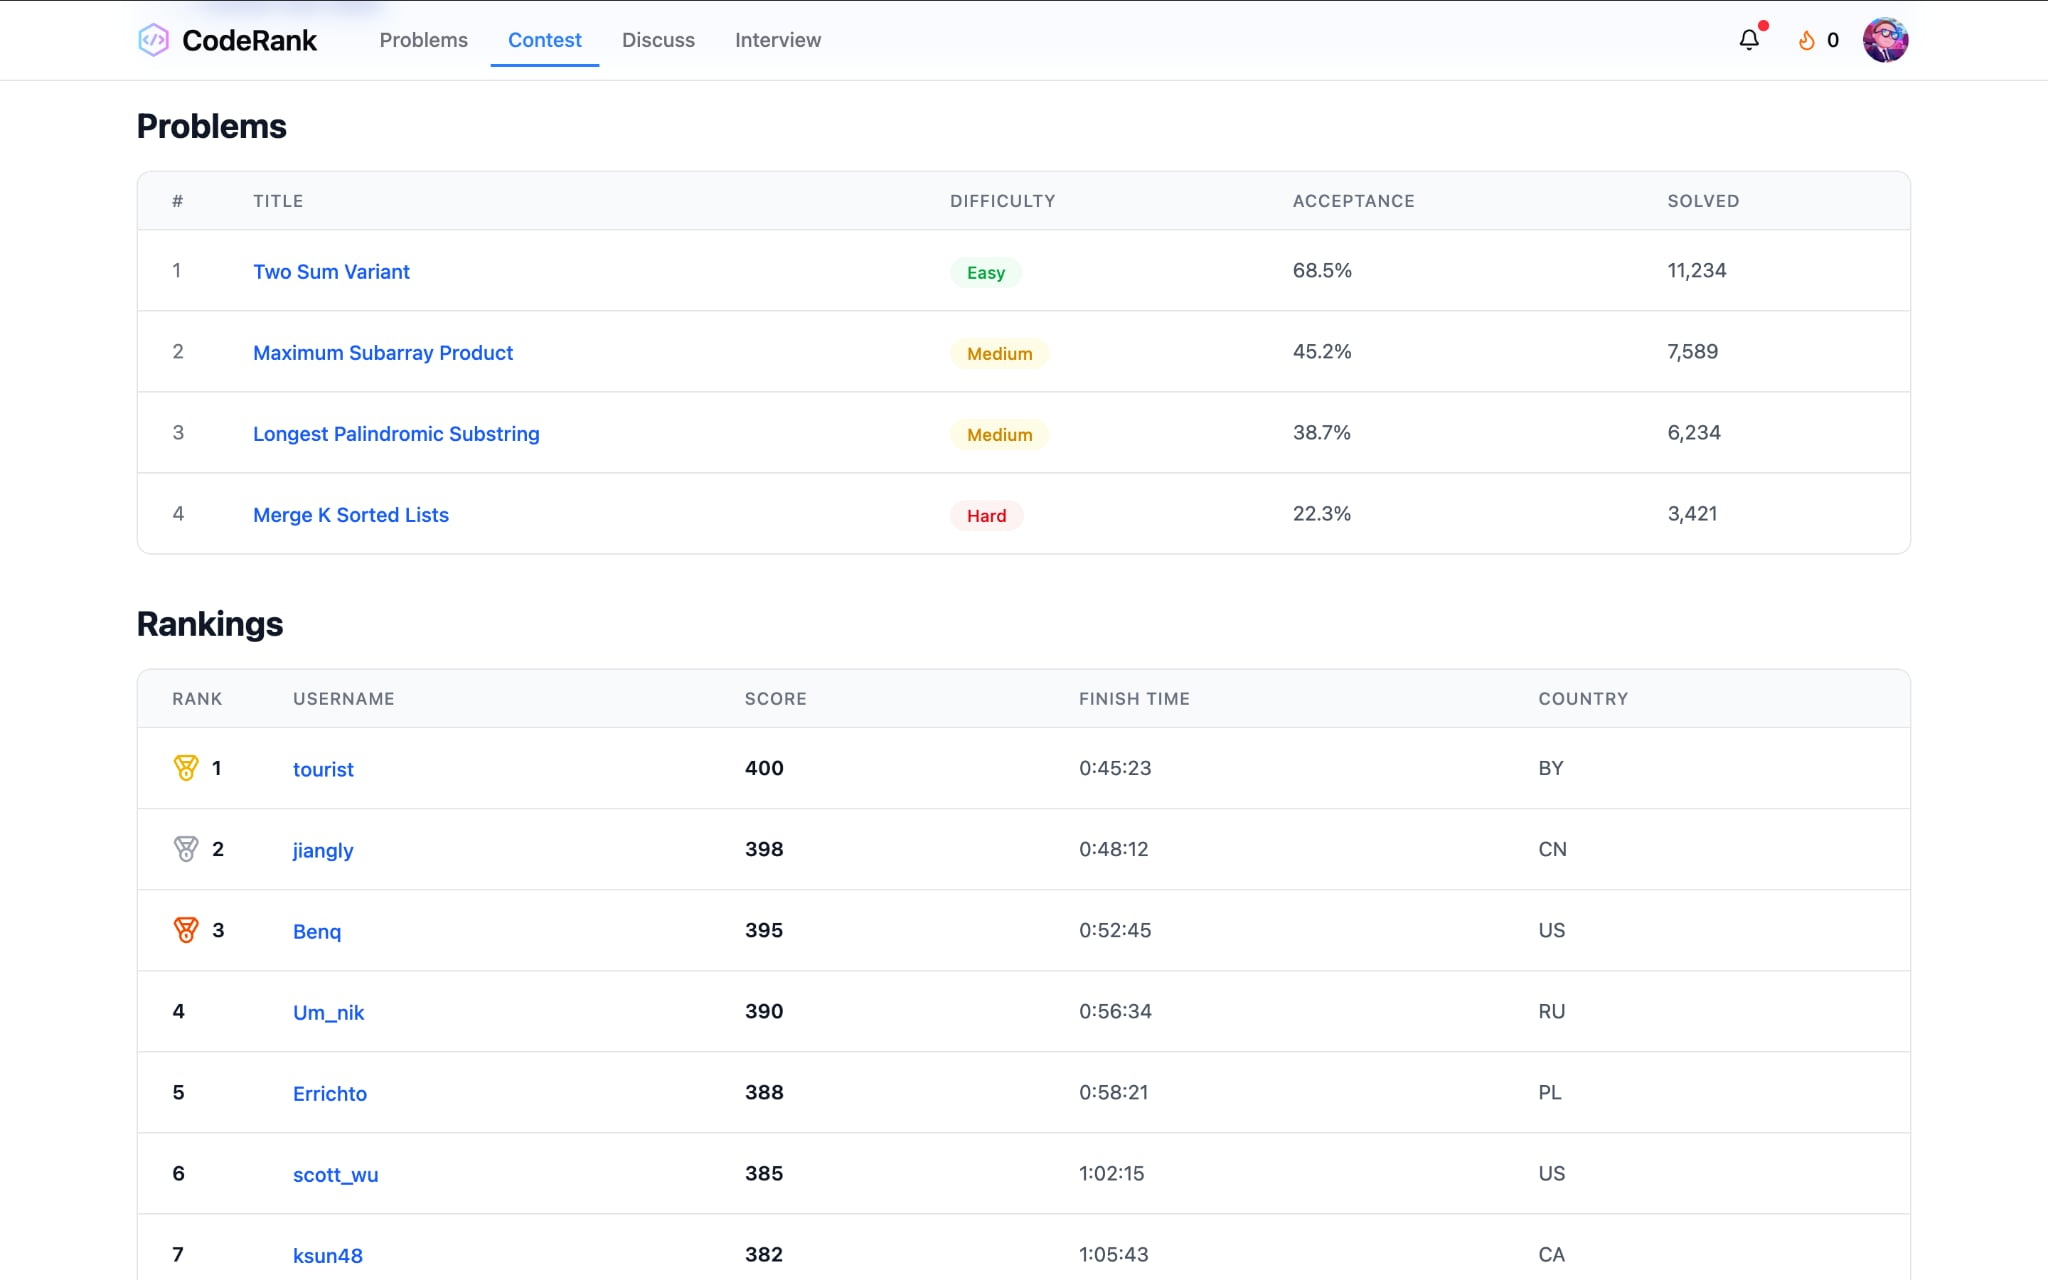
\includegraphics[width=1\textwidth]{Contents/Chapter 3/Wireframe/Primary User/contest-4.jpeg}
    \vspace{0.6cm}
    \caption{Contest Detail}
\end{figure}

In order to create a custom contest, the user can click on the \textbf{Create Contest} button in the Contest List page. Here, they can enter the contest name, select problems to include in the contest, set the start and end time, and define other contest settings.
\begin{figure}[H]
    \centering
    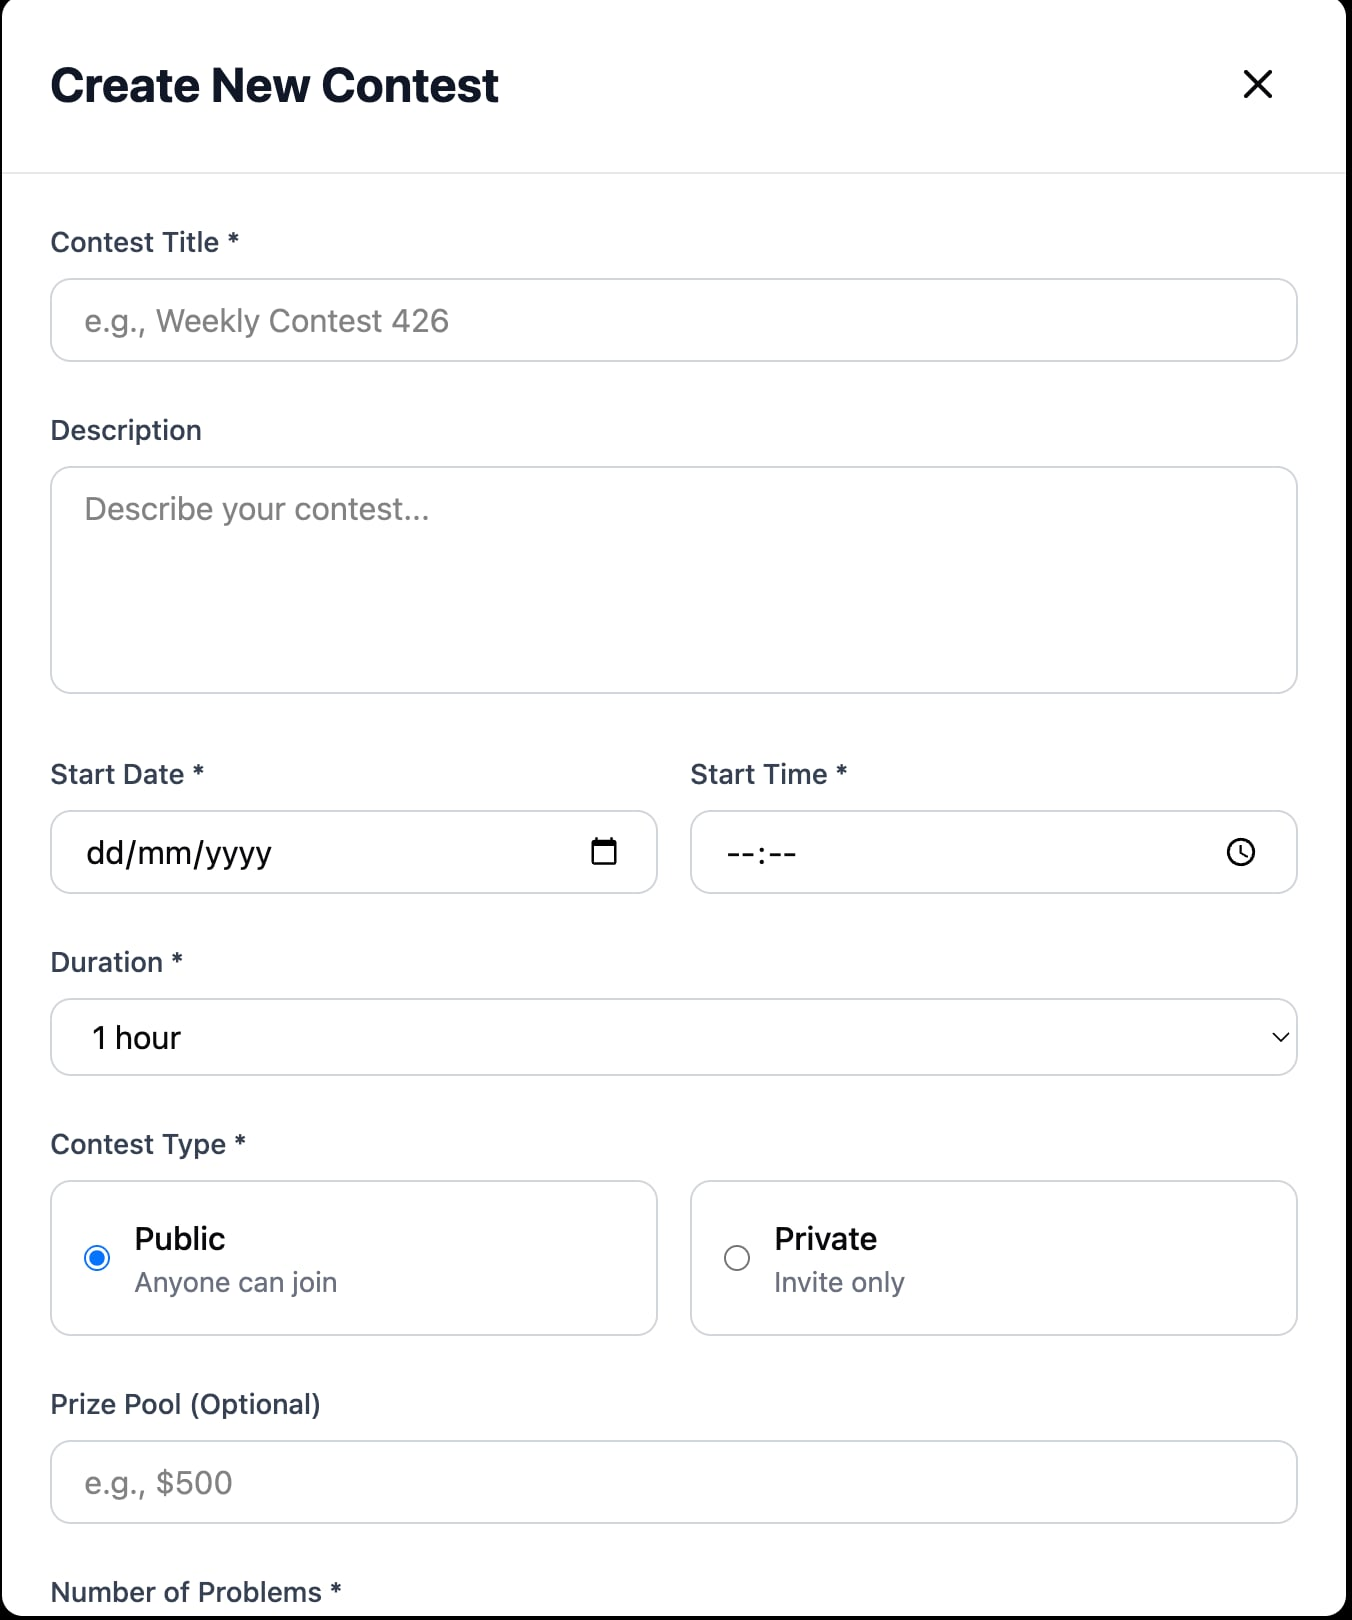
\includegraphics[width=1\textwidth]{Contents/Chapter 3/Wireframe/Primary User/contest-2.jpeg}
    \vspace{0.6cm}
    \caption{Contest Creation}
\end{figure}

\subsubsection*{Interview Preparation}
Primary users can access the Interview Preparation feature from the main navigation menu. The Interview Preparation feature provides users with a curated list of coding problems and resources specifically designed to help them prepare for technical interviews. In the Interview Preparation page, there will be a conversation history section on the left side, displaying a list of previous interview preparation sessions. Users can select a session to view the details and continue their preparation or create a new session by clicking the \textbf{New Conversation} button.
\begin{figure}[H]
    \centering
    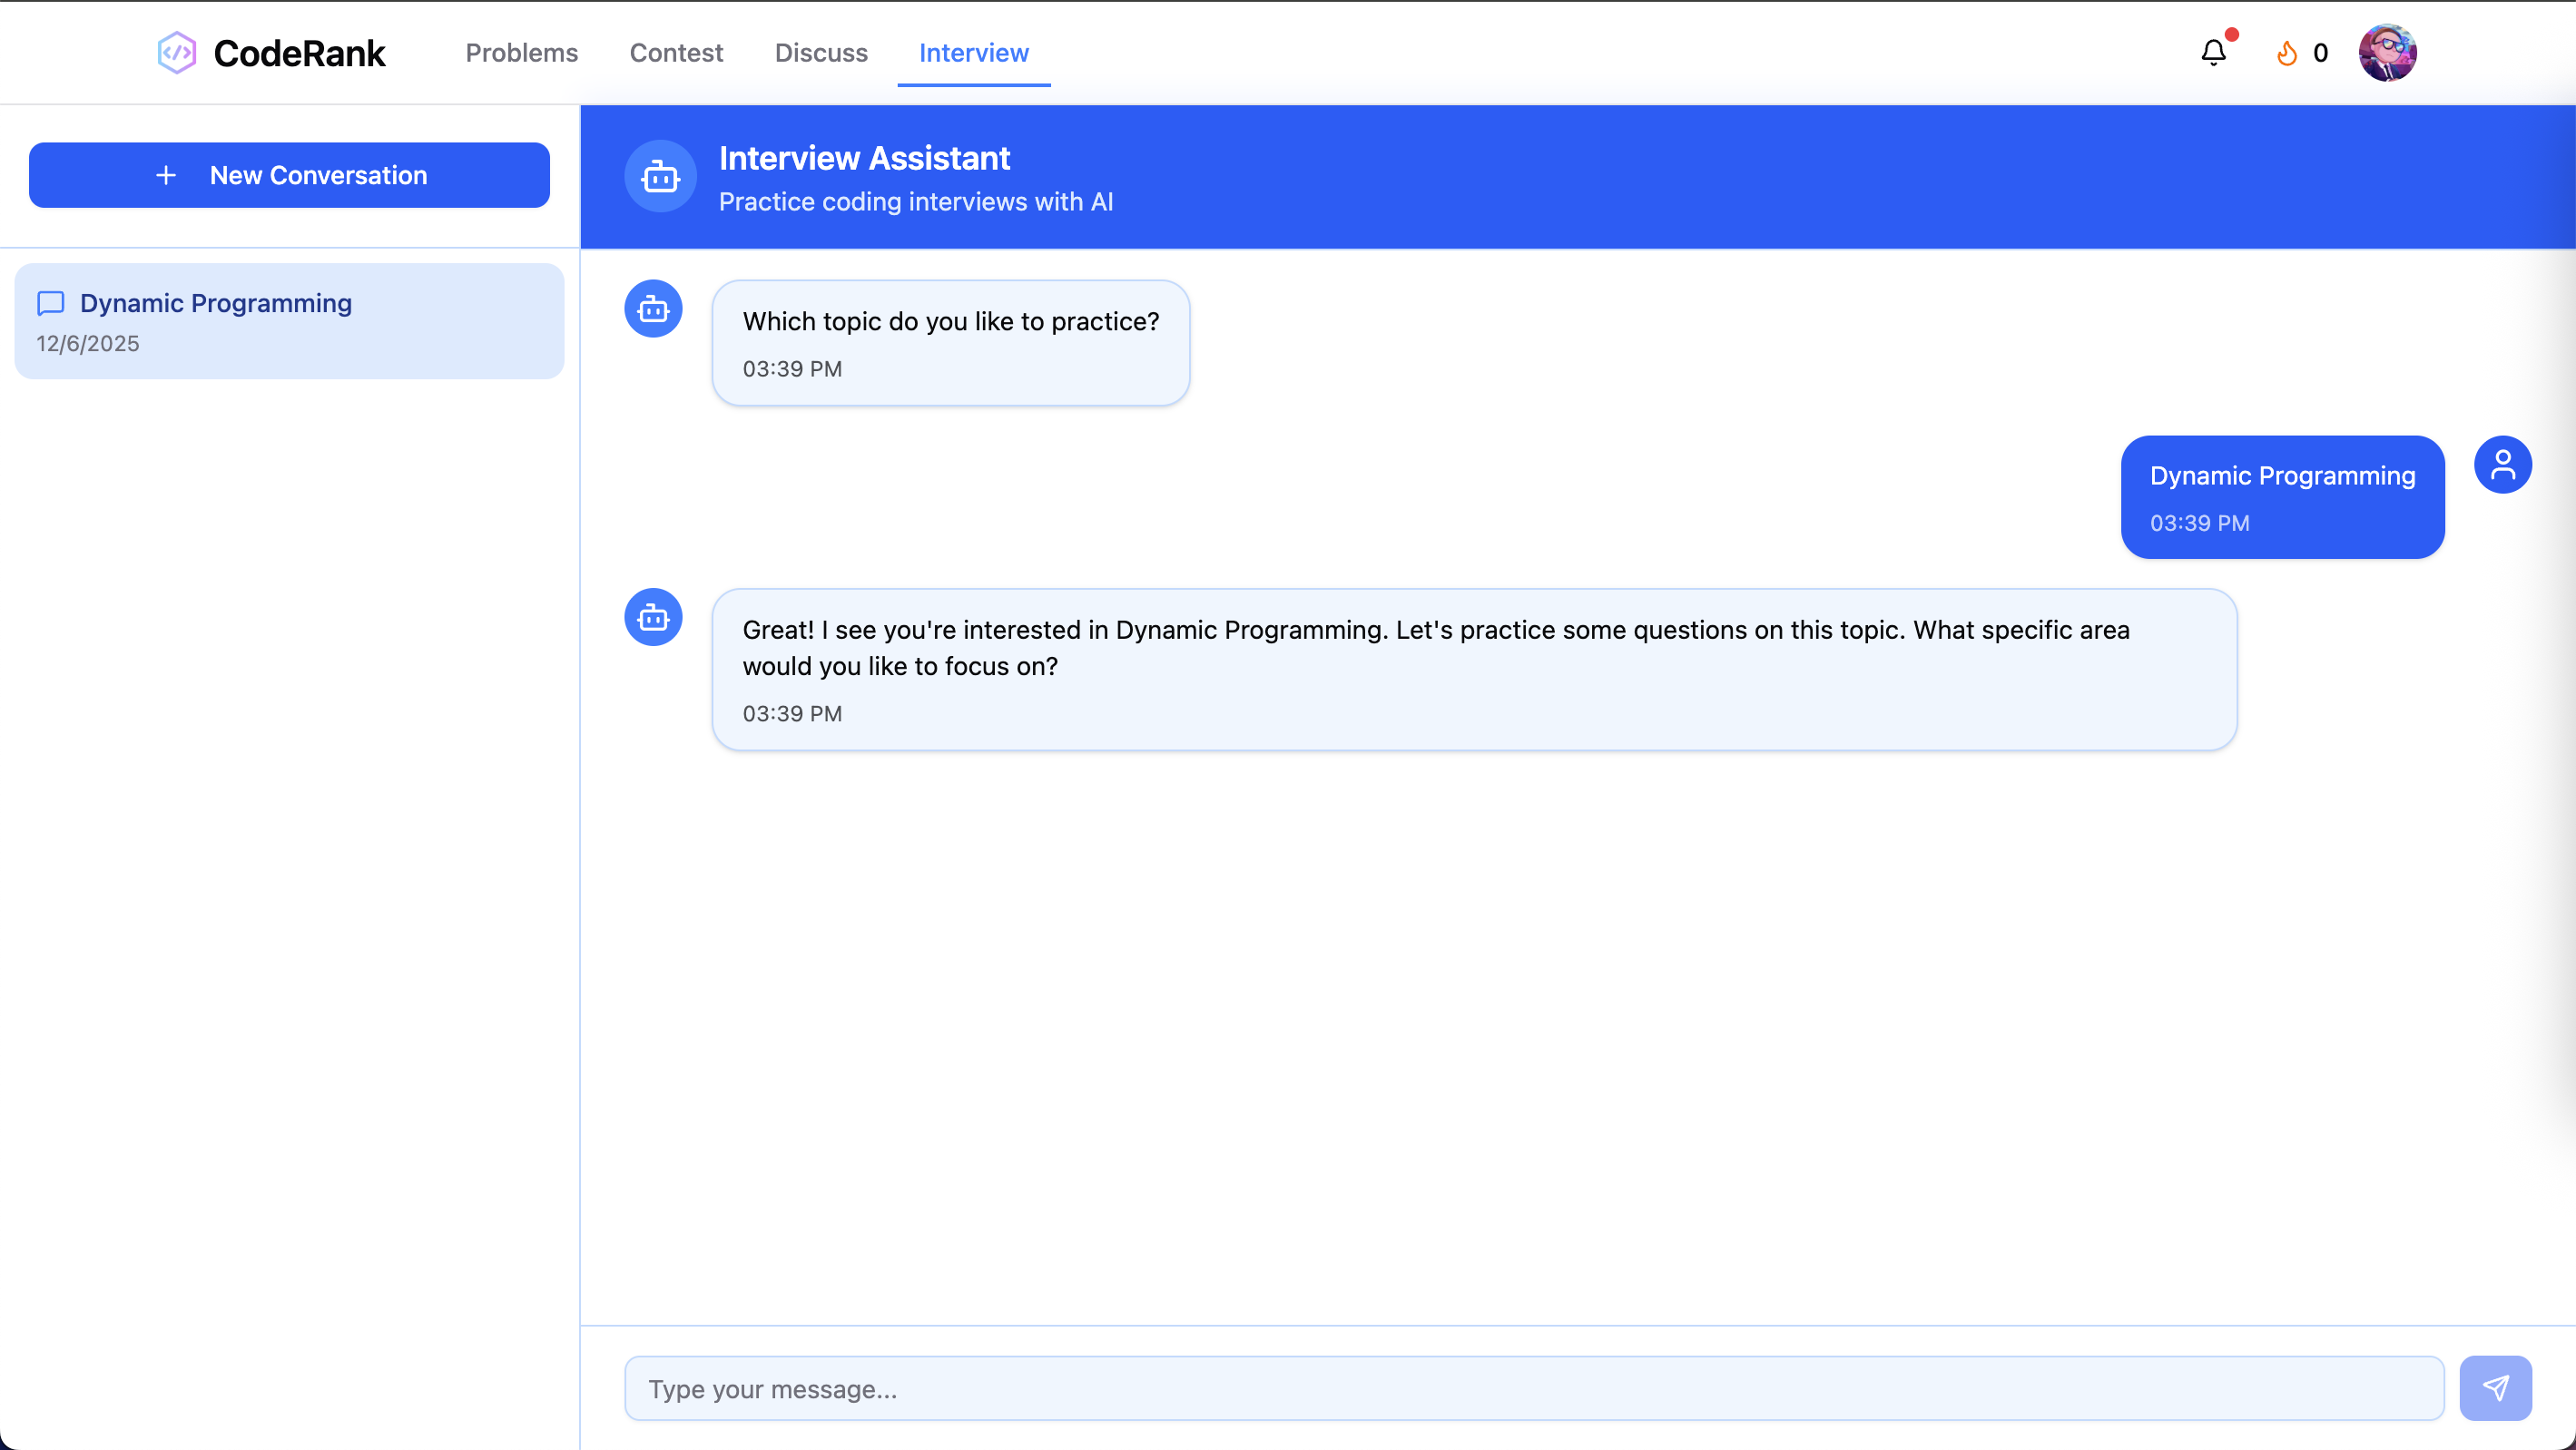
\includegraphics[width=1\textwidth]{Contents/Chapter 3/Wireframe/Primary User/inteview-1.png}
    \vspace{0.6cm}
    \caption{Interview Preparation Page}
\end{figure}

\subsection{Moderator/Admin flow}

After logging in as a Moderator/Admin, the user will be directed to the Moderator/Superadmin Dashboard. This dashboard provides an overview of key metrics and functionalities available to moderators and administrators, allowing them to manage the platform effectively.
\begin{figure}[H]
    \centering
    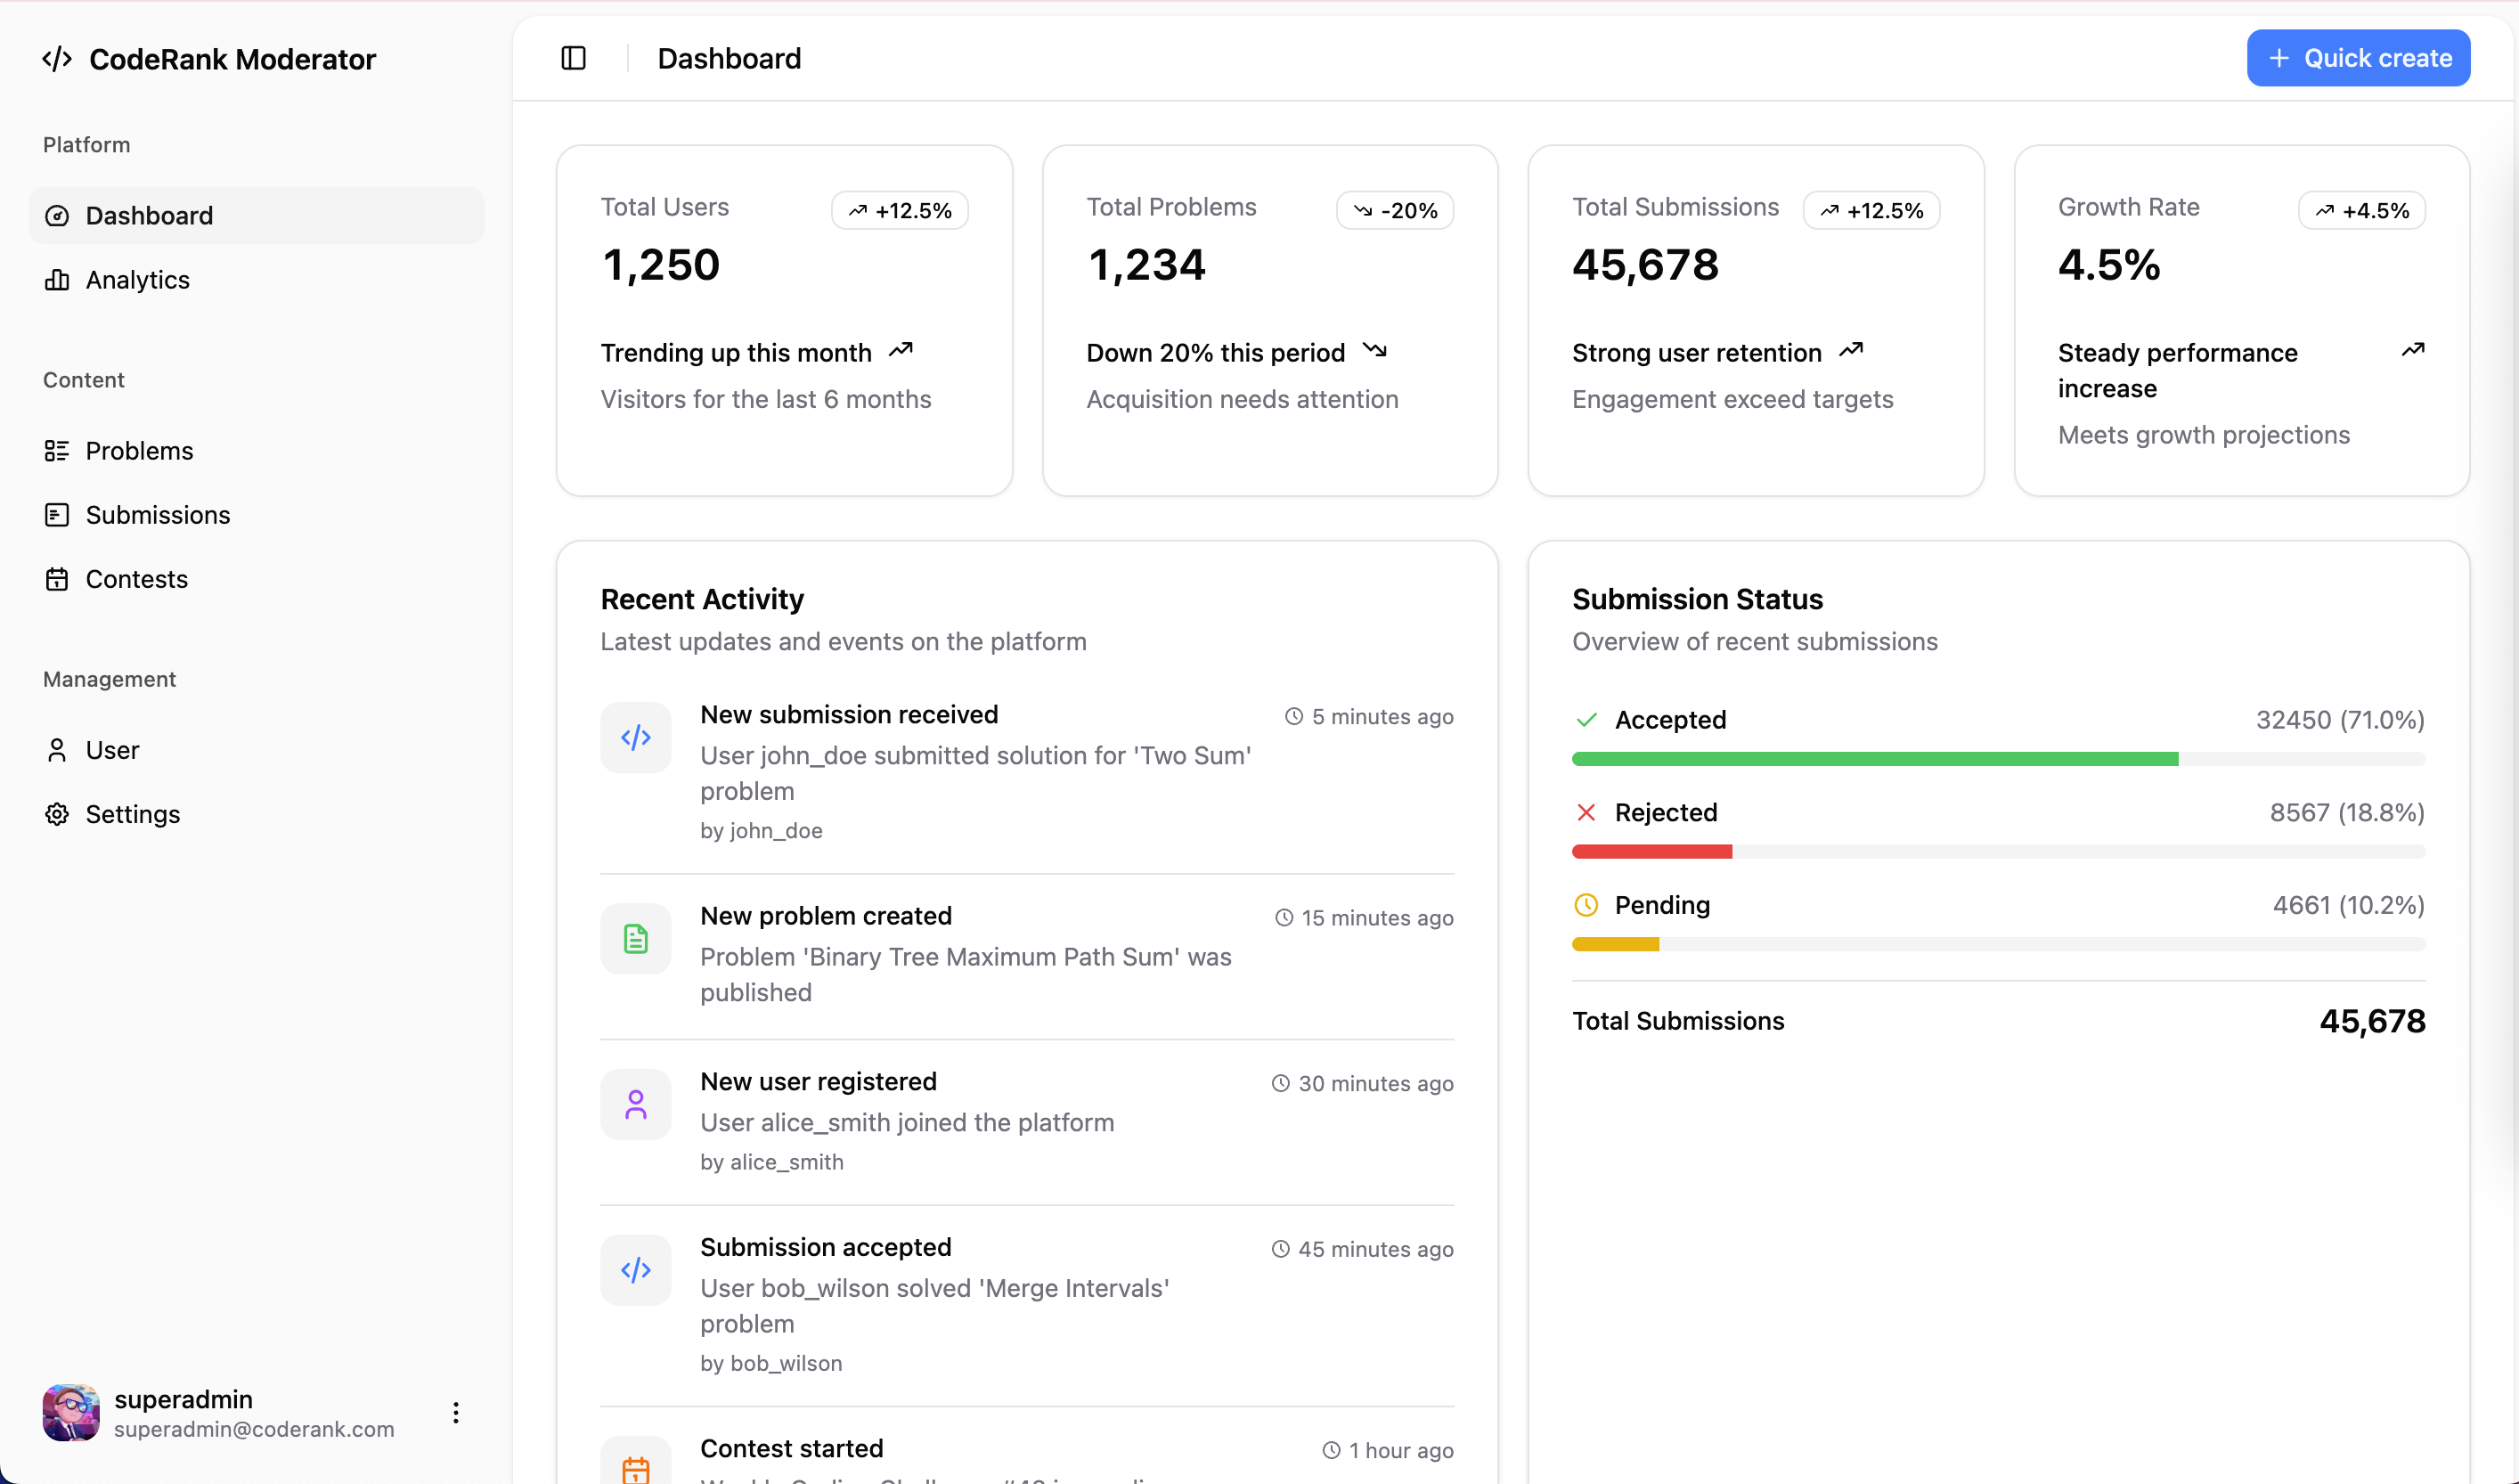
\includegraphics[width=1\textwidth]{Contents/Chapter 3/Wireframe/Admin/admin-1.png}
    \vspace{0.6cm}
    \caption{Moderator Dashboard}
\end{figure}

Moderators/Admins can manage problem create requests submitted by another Moderator by navigating to the Problems sidebar, where a list of all problem requests is displayed along with their Difficulty level, color-coded for quick reference (Easy, Medium, Hard). In addition, this list is paginated, showing 10 items per page to ensure clear and efficient navigation.
\begin{figure}[H]
    \centering
    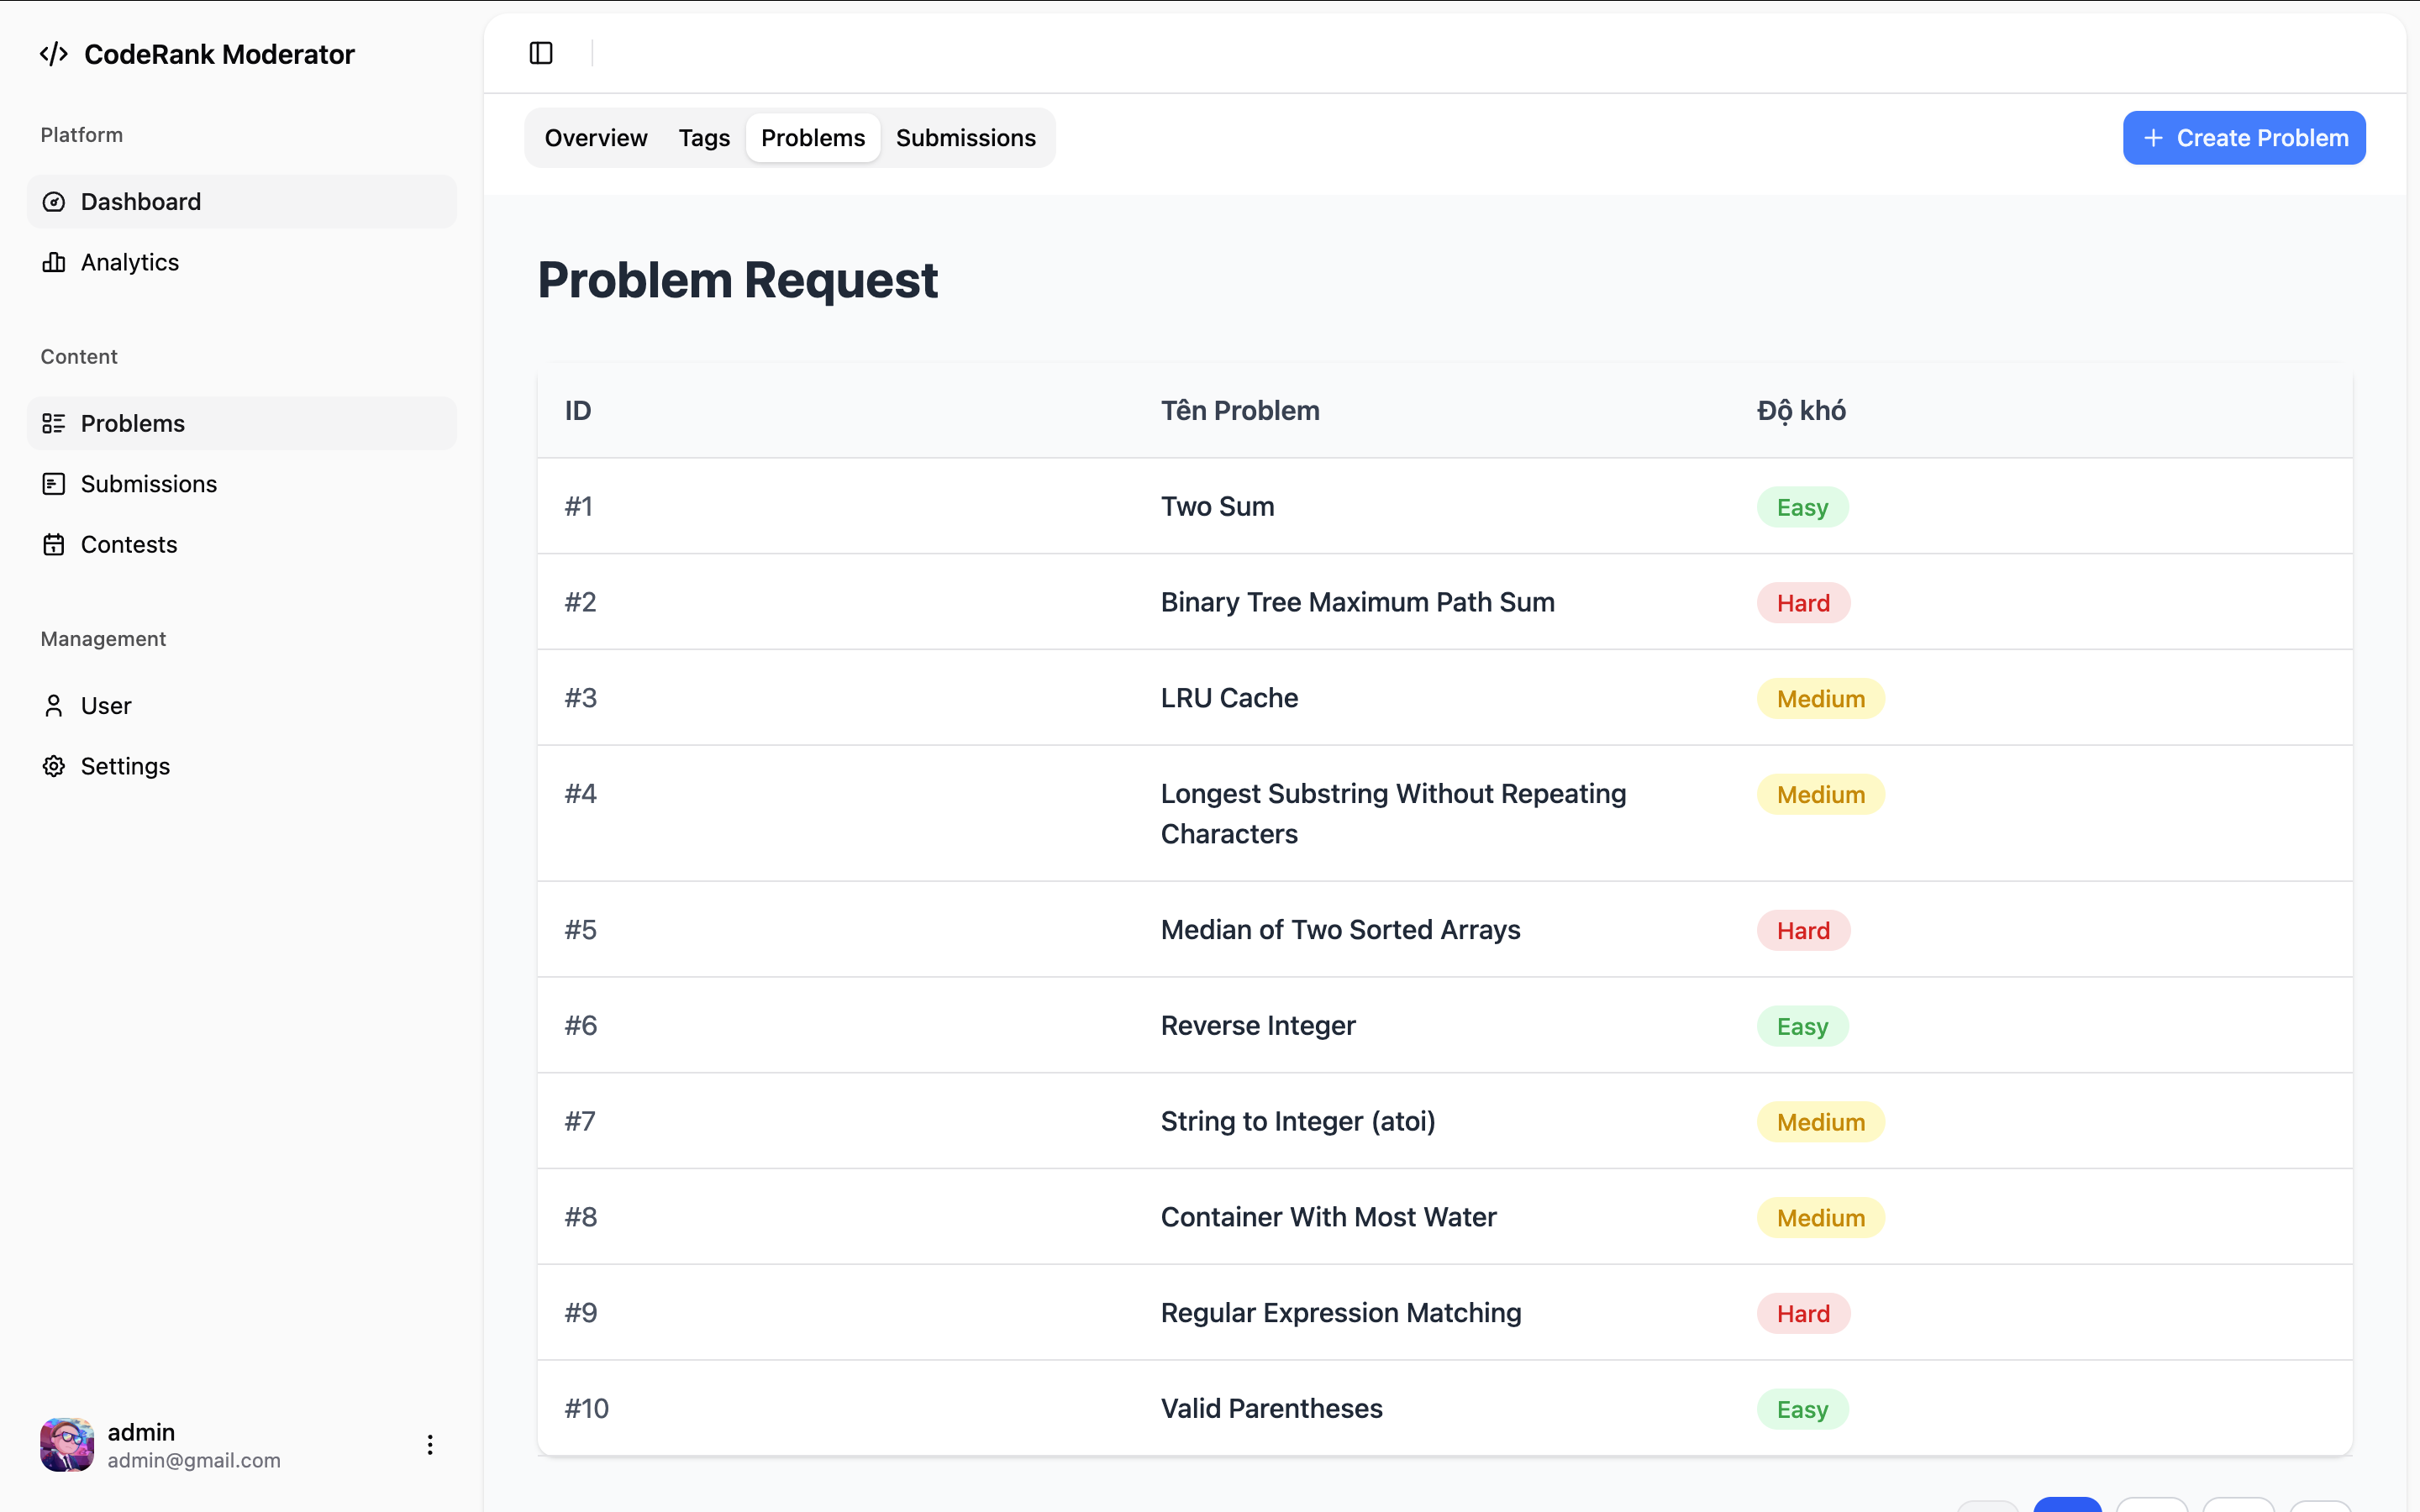
\includegraphics[width=1\textwidth]{Contents/Chapter 3/Wireframe/Admin/Problem_request_list.png}
    \vspace{0.6cm}
    \caption{Problem Request List}
\end{figure}


A “Create Problem” button is positioned at the top-right corner of the interface, allowing users to quickly submit a new problem request. When this button is clicked, a creation modal appears centered on the screen, enabling Moderators/Admins to input all necessary details, in which user is required to fill in fields such as Problem Name, Difficulty level, Topic, and any other relevant information needed to define the problem.
\begin{figure}[H]
    \centering
    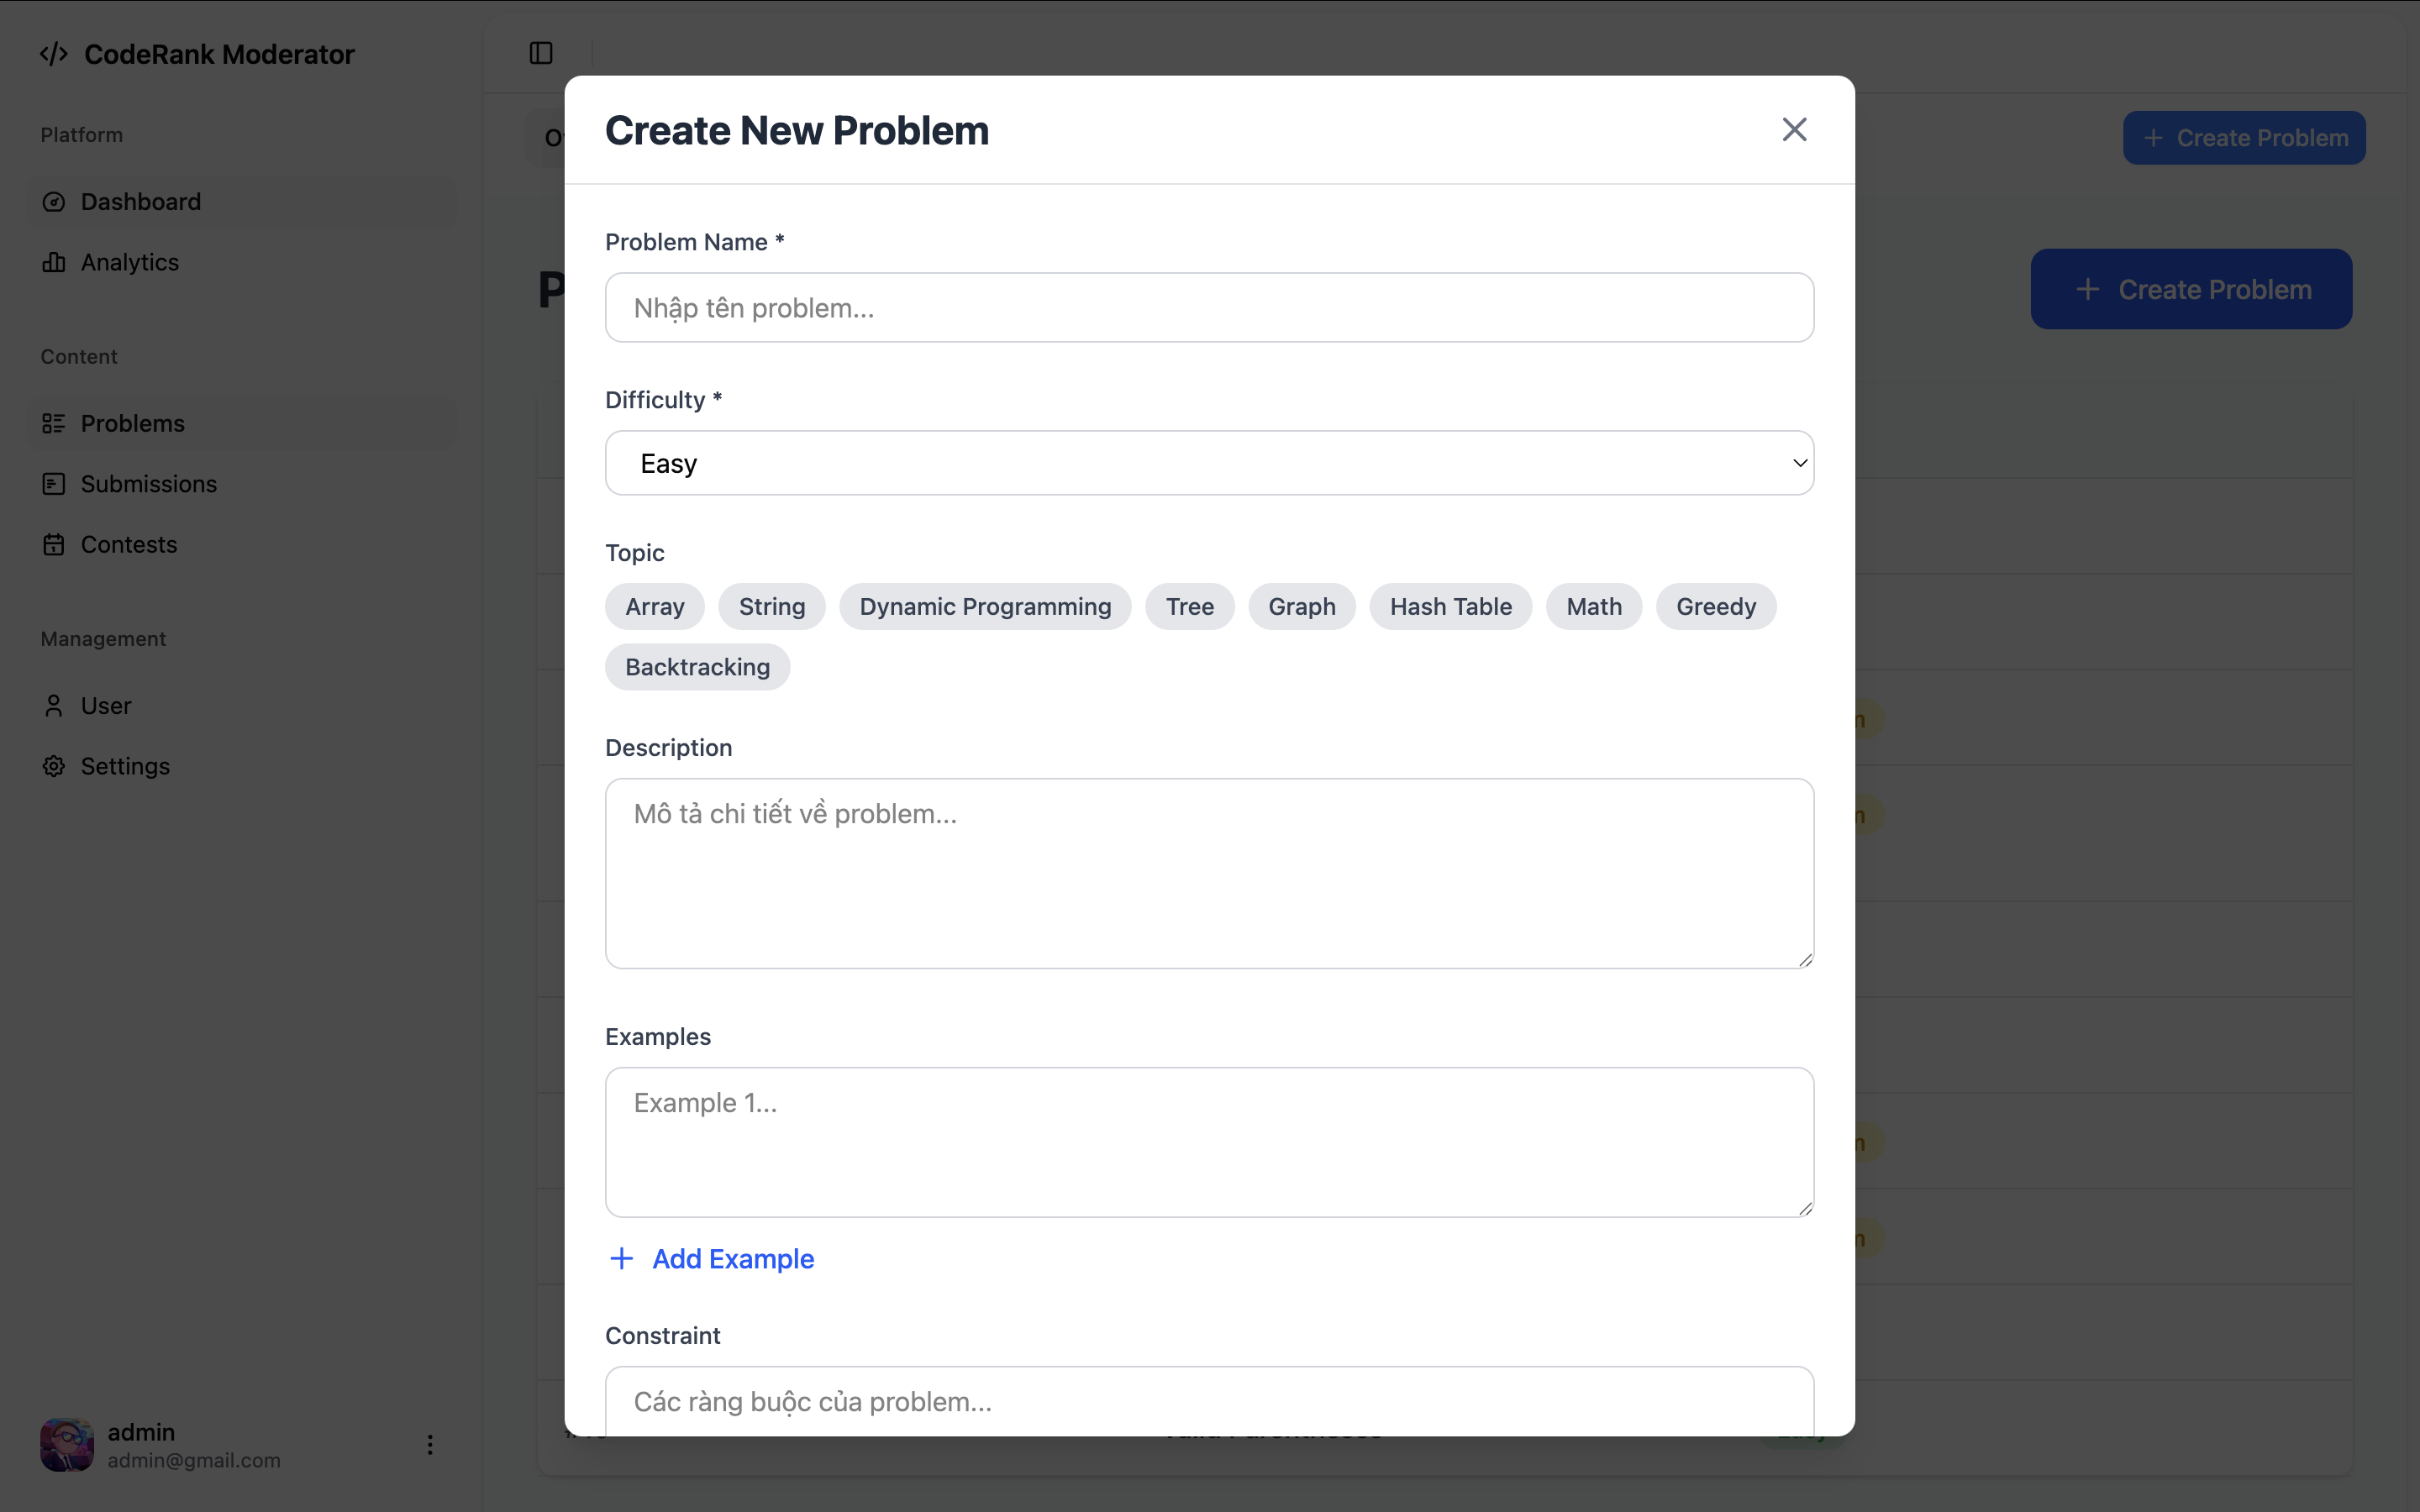
\includegraphics[width=1\textwidth]{Contents/Chapter 3/Wireframe/Admin/Problem_request_modal.png}
    \vspace{0.6cm}
    \caption{Problem Request Create Modal}
\end{figure}

Users can also review any problem request by clicking on its corresponding row, which navigates them to the detailed view of that request. This page displays the full information of the problem request. All Moderators can view these details, but only Admins have permission to take action. At the bottom of the page, Admins can choose to Approve or Deny the request via two dedicated buttons.

\begin{figure}[H]
    \centering
    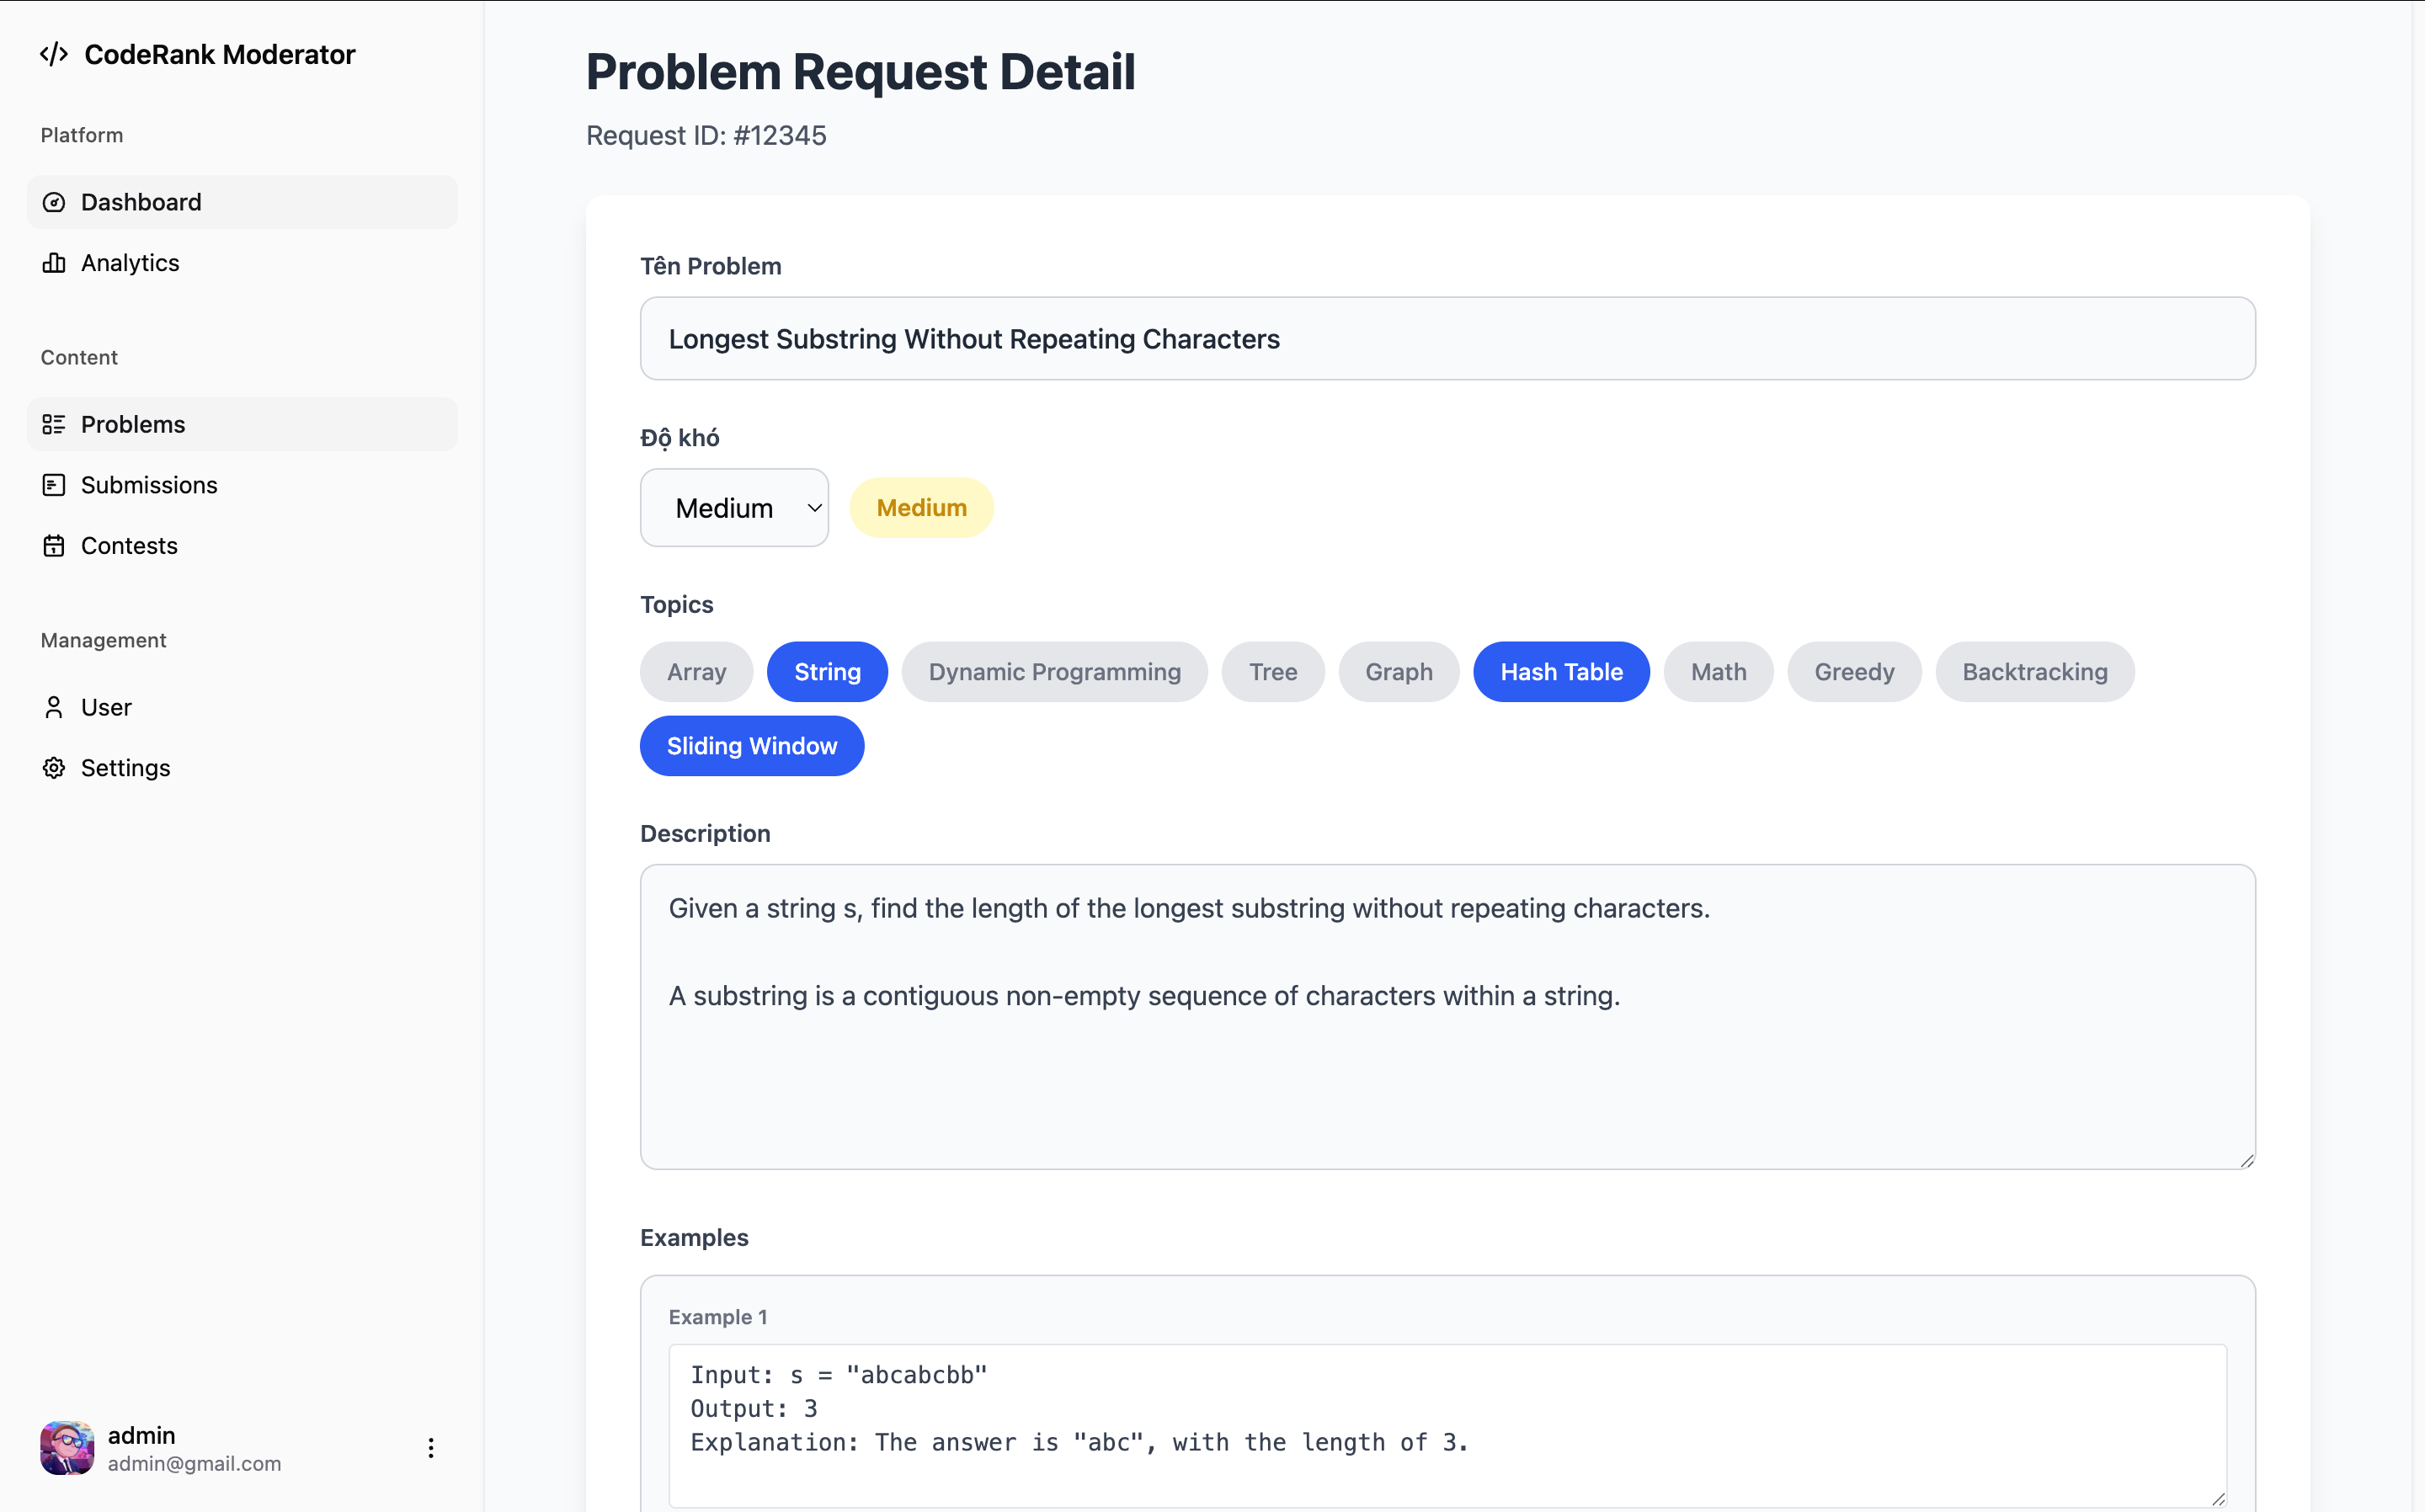
\includegraphics[width=1\textwidth]{Contents/Chapter 3/Wireframe/Admin/Problem_detail_1.png}
    \vspace{0.6cm}
    \caption{Problem Request Detail \#1}
\end{figure}

\begin{figure}[H]
    \centering
    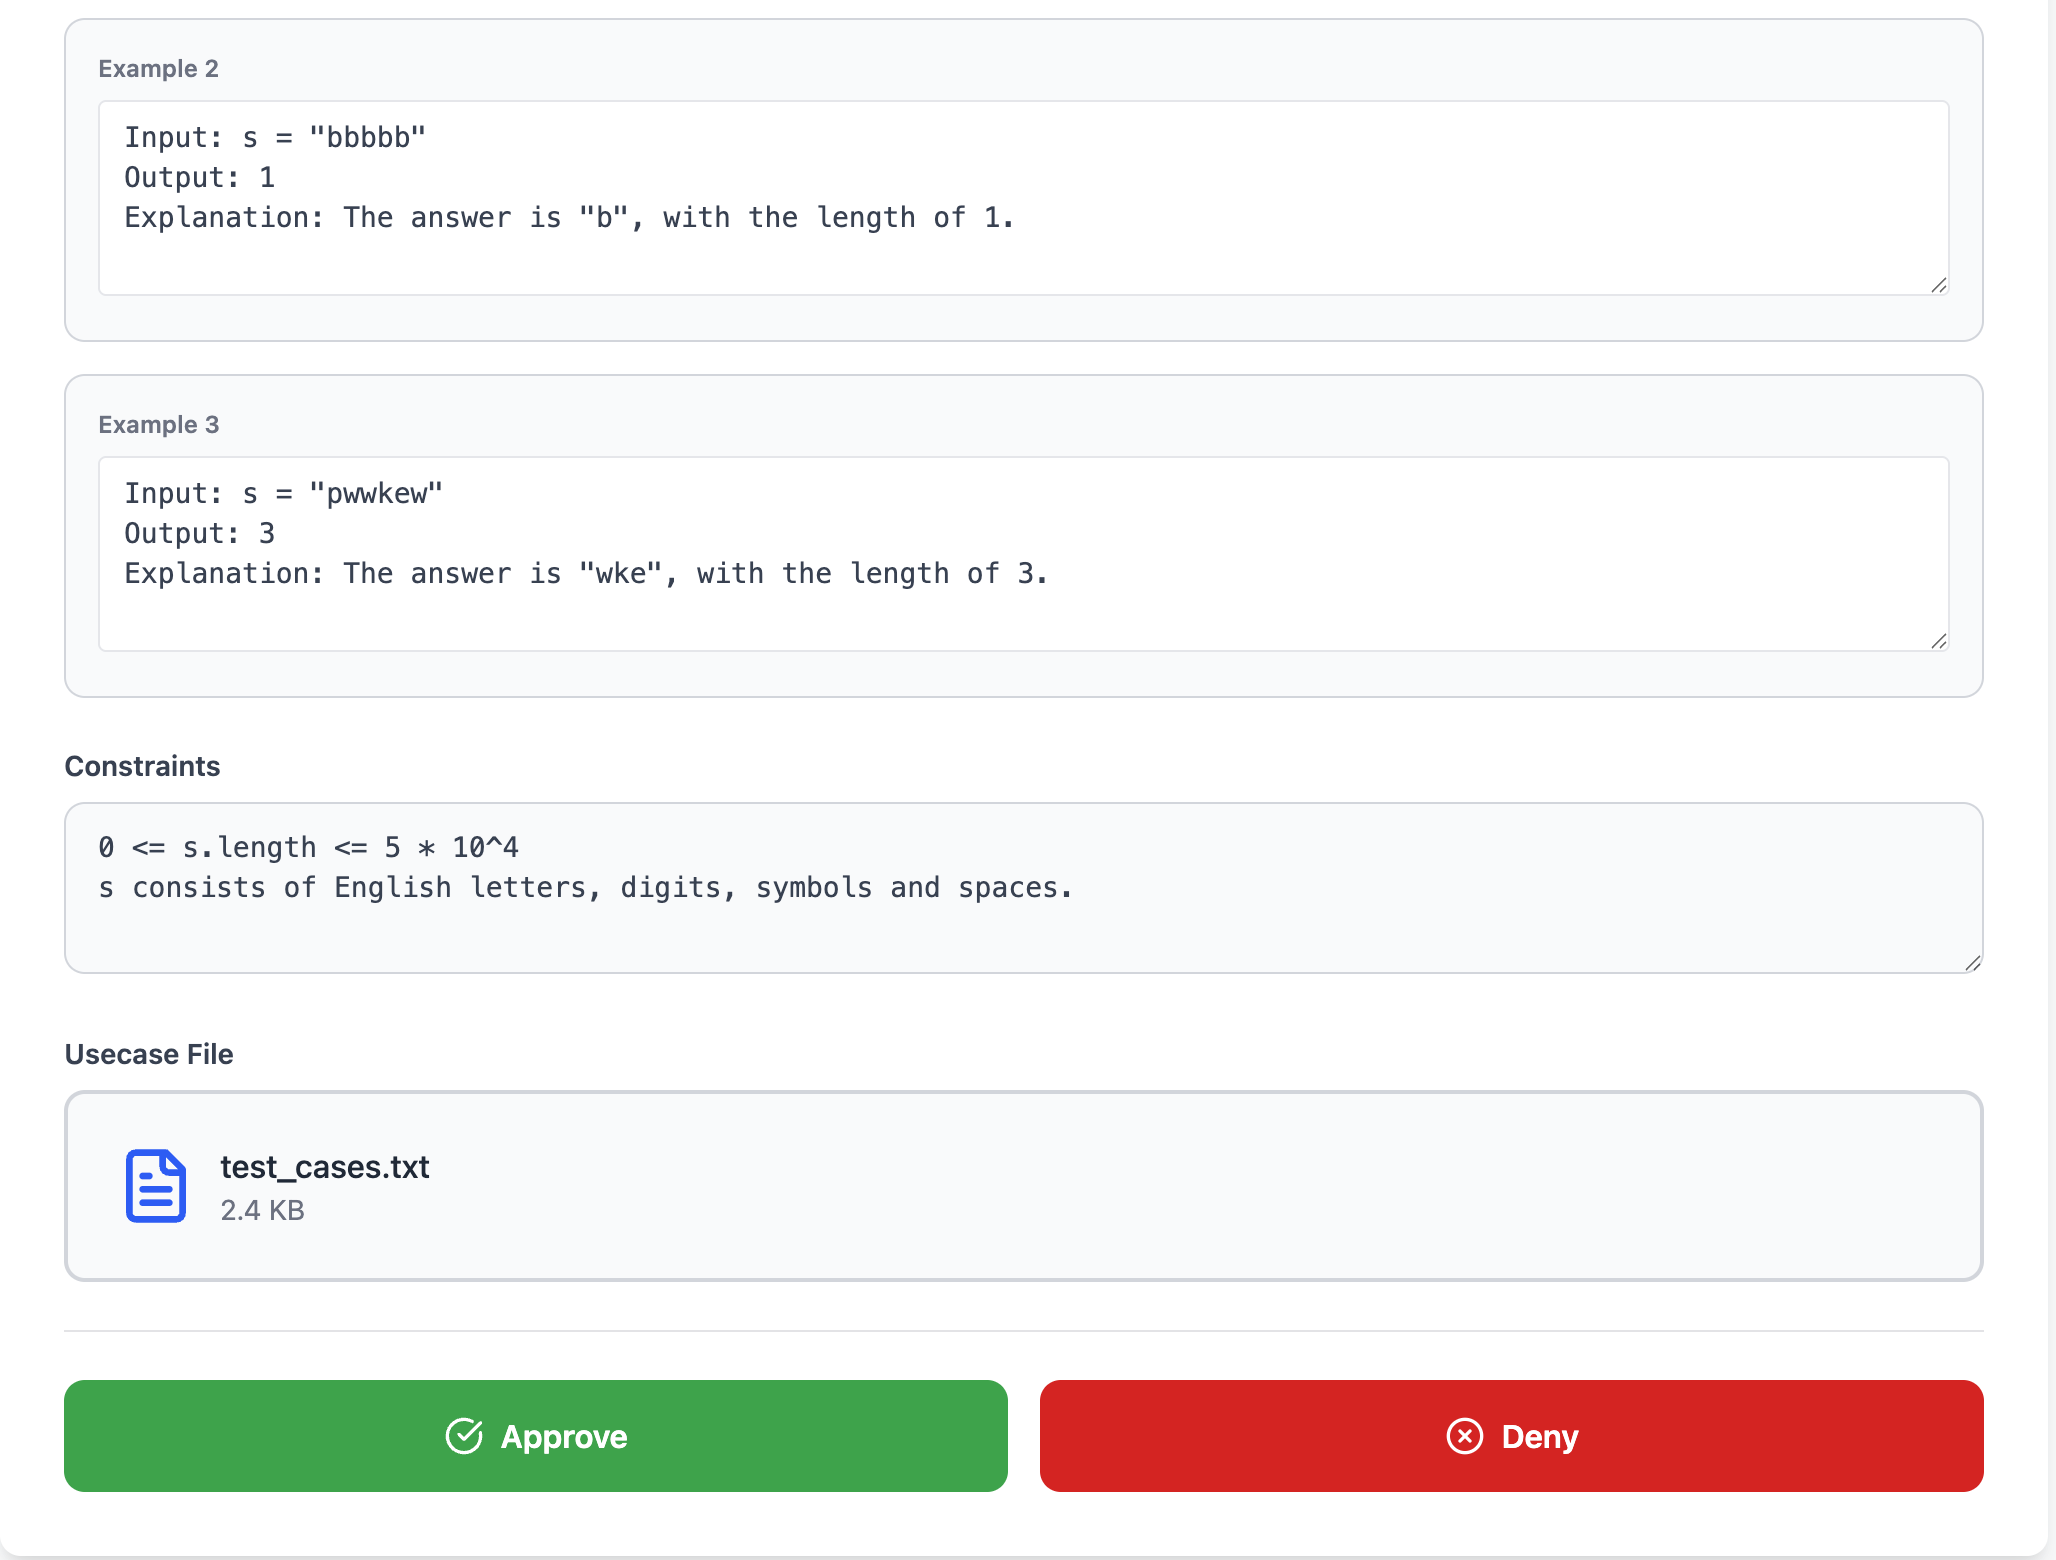
\includegraphics[width=1\textwidth]{Contents/Chapter 3/Wireframe/Admin/Problem_detail_2.png}
    \vspace{0.6cm}
    \caption{Problem Request Detail \#2}
\end{figure}

If an Admin selects Deny, a confirmation modal appears, requiring them to provide a mandatory explanation for the denial before the action can be confirmed.
\begin{figure}[H]
    \centering
    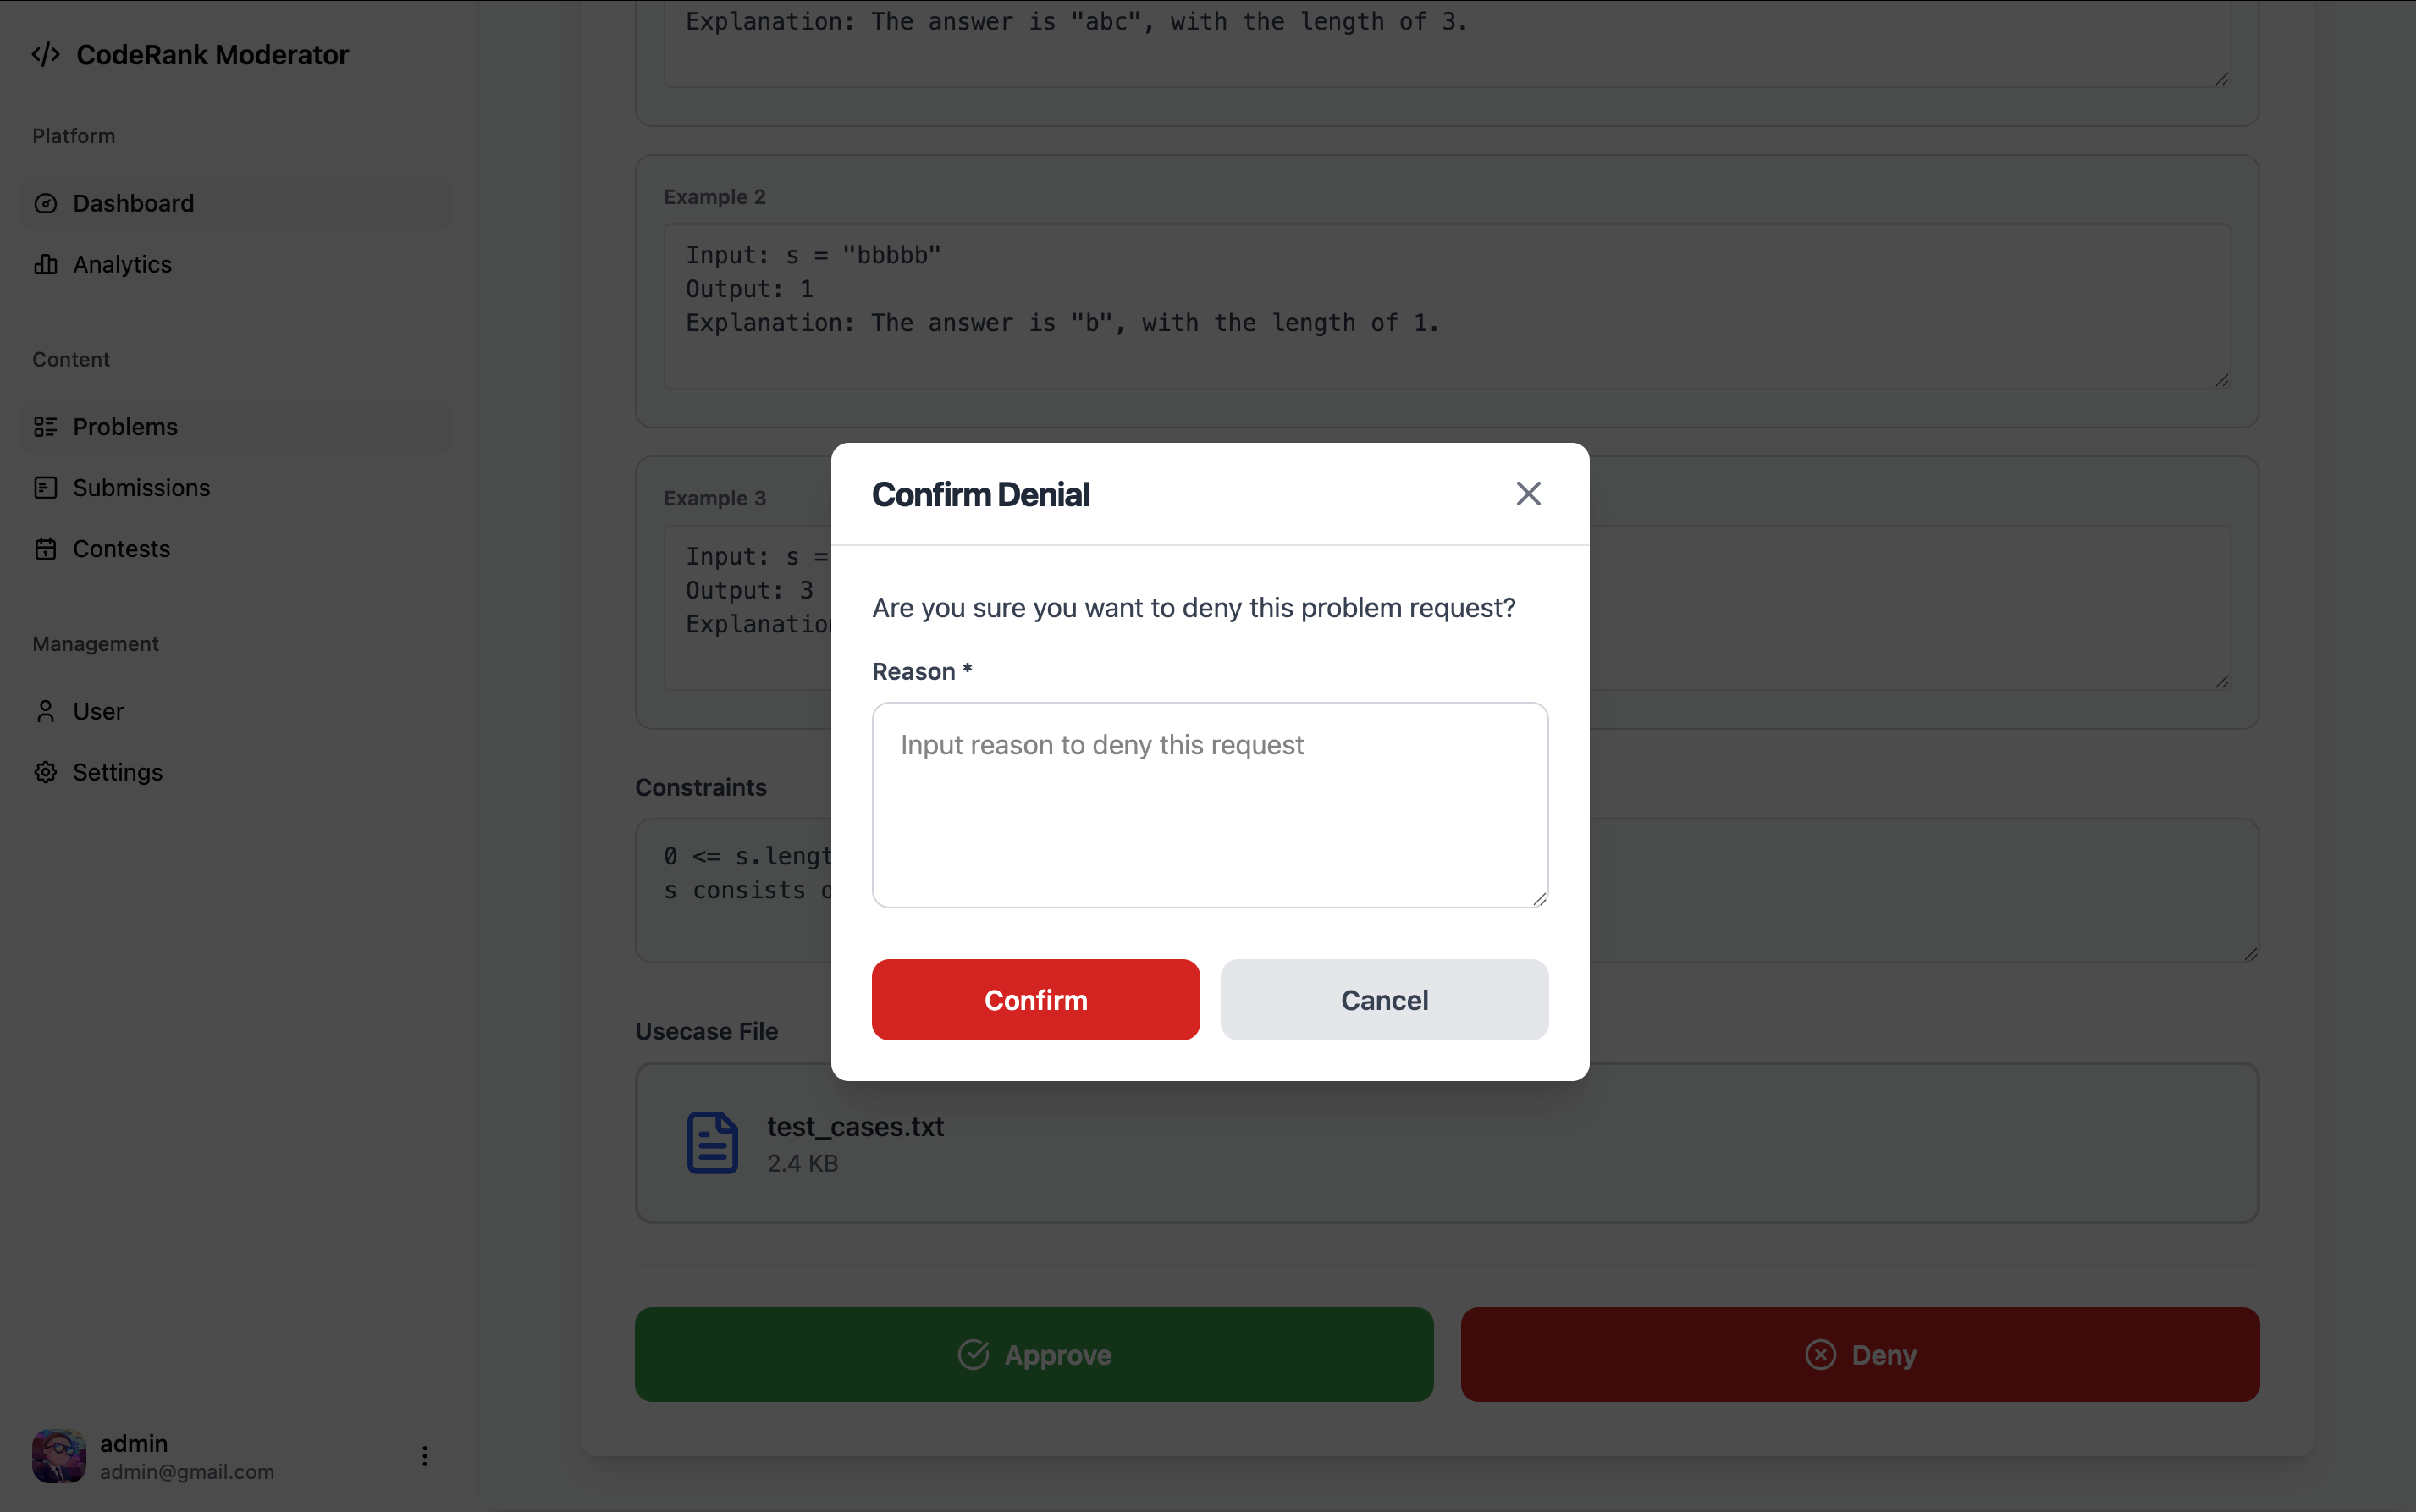
\includegraphics[width=1\textwidth]{Contents/Chapter 3/Wireframe/Admin/Problem_confirm_modal.png}
    \vspace{0.6cm}
    \caption{Problem Request Confirm Modal}
\end{figure}

